%% Chapter 13 — MLOps and Deployment Automation
\setcounter{chapter}{12}
\chapter{MLOps and Deployment Automation}
\chaptersubtitle{Registries, pipelines, canaries, and shadows — how a deploy becomes the most boring sentence in engineering}

\begin{calloutbox}{tbbblue}{tbbbluefill}
{\normalsize\bfseries\color{tbbblue}Learning objectives}\par\vspace{3pt}
\begin{tbbitemize}
  \item Diagnose a bad deploy as \textbf{missing institutions} (versioned releases, pipelines, gradual exposure) rather than personal carelessness — and price the difference in bad user-minutes.
  \item Operate a \textbf{model registry}: the release triple (weights + config + image digests), gate evidence, lineage, stage aliases — and rollback as a rehearsed pointer flip.
  \item Build \textbf{model CI/CD}: the three lanes (PR checks, merge-to-registry, promote-with-canary), why model CI differs from app CI, and GitHub Actions mechanics including a self-hosted GPU runner.
  \item Choose deployment strategies by the \textbf{question each answers}: rolling ("does it boot?"), blue/green ("can I undo instantly?"), canary ("is it broken?"), A/B ("is it better?"), shadow ("what would it have done?").
  \item Design a \textbf{canary analysis} for generative models — SLO clauses plus guardrail proxies, session-consistent splits, auto-promote/auto-retreat — and say what it checks that the offline gate cannot.
  \item Place \textbf{managed endpoints} (SageMaker, Vertex AI) on the operator ladder: what they run, what they charge, and what always stays yours.
\end{tbbitemize}
\end{calloutbox}

\vspace{2.5pt}

\begin{calloutbox}{tbbteal}{tbbtealfill}
{\normalsize\bfseries\color{tbbteal}Key terms}\par\vspace{3pt}
bad user-minutes · model registry · release triple · lineage · stage alias · promotion / rollback · CI/CD · GitHub Actions · self-hosted runner · OIDC · golden requests · quick gate vs. full gate · progressive delivery · rolling · blue/green · canary · automated analysis · guardrail metric · A/B test · shadow / dark launch · Argo Rollouts · managed endpoint · deployment guardrails · DORA metrics
\end{calloutbox}

\vspace{2.5pt}

\begin{calloutbox}{tbblightgray}{tbbboxfill}
{\normalsize\bfseries\color{tbbink}Chapter outline}\par\vspace{3pt}
\textbf{13.1} The Friday deploy — and the most expensive missed server in history    \textbf{13.2} The registry: versions with meaning    \textbf{13.3} The pipeline: every promise, checked by a machine    \textbf{13.4} Meeting real traffic: rolling, blue/green, canary, A/B, shadow    \textbf{13.5} Managed endpoints: the operator ladder, completed    \textbf{13.6} Lab: build the pipeline, then fail to break production — followed by a summary, exercises, and further reading.
\end{calloutbox}

\section{The Friday Deploy — and the Most Expensive Missed Server in History}

Chapter 12 ended on an honest embarrassment: a fleet that breathes, a bill that closes — and every single improvement shipped by \textbf{a human typing kubectl at a laptop}. The course has been quietly building the alternative for weeks (digests, stores, gates, probes, canary fields), but nothing has yet assembled the pieces, and un-assembled pieces do not protect anyone. Here is what that looks like, on a Friday, at six in the evening — every detail of which your team is currently capable of reproducing:

\begin{terminalbox}
\begin{Verbatim}[breaklines=true,breakanywhere=true,fontsize=\small,formatcom=\color{tbbtermfg},codes=\tbbcodeactive]
# friday 18:07. v10-awq passed the offline gate this afternoon.
$ kubectl set env deploy/chat MODEL_URI=s3://models/chat/v10-awq/
# 18:12  rolling update complete. probes green. weekend, here we come.
# 18:19  support: "answers keep cutting off mid-sentence??"
$ kubectl get pods; curl :8000/metrics | grep -E "ttft|error"
#        pods Ready. TTFT p99 0.44s. errors 0.0%. ...all GREEN.
# 18:31  more tickets. decision: roll back. ...roll back to WHAT?
$ history | grep MODEL_URI      # archaeology. Slack. more grep.
# 18:43  found it: v9-int4. re-deploy. 18:56: healthy.
#
# the bug: v10's bundled generation_config.json shipped
# max_tokens: 256 (v9: 1024). the model was FINE. the gate never
# noticed - it scores teacher-forced eval, it never GENERATES.
# damage: 37 minutes x 100% of users. mean answer: 211 -> 54 tokens.
\end{Verbatim}
\end{terminalbox}
\figcaption{Exhibit 13-A  The Friday deploy. Nothing crashed; every dashboard stayed green; the model itself was perfect. A config file that traveled outside the release cut every answer to a quarter of its length for 37 minutes — and the rollback took twelve minutes of shell-history archaeology because nobody could say what "before" was.}

Resist the first diagnosis your organization will offer — \textit{"the engineer should have checked max\_tokens"} — because it is both true and useless. Individuals err at a roughly constant rate; systems decide how much each error costs. Read the exhibit again as an auditor rather than a judge and three \textbf{missing institutions} appear. Nobody could answer \textit{"what was live before?"} in less than twelve minutes — a \textbf{versioning} failure (the store had immutable bytes; nothing recorded which bytes, with which config, constituted the running release). The gate scored the model but never \textit{generated with the shipped config} — a \textbf{pipeline} failure (checks ran on what was convenient to check, not on the artifact as deployed). And v10 met 100\% of users in its first second — an \textbf{exposure} failure (no gradual contact with reality, no automated retreat). Fix the engineer and Friday repeats with a different engineer. Fix the three institutions and Friday becomes Figure 13-1's second timeline: the same bug, caught by a 10\% canary's answer-length guardrail in under five minutes, auto-retreated, evidence filed on the PR — \textbf{0.5 bad user-minutes instead of 37}, a 74× reduction, and nobody's weekend involved.

\begin{tbbfigure}
  \adjustbox{max width=0.94\linewidth,max totalheight=0.46\textheight}{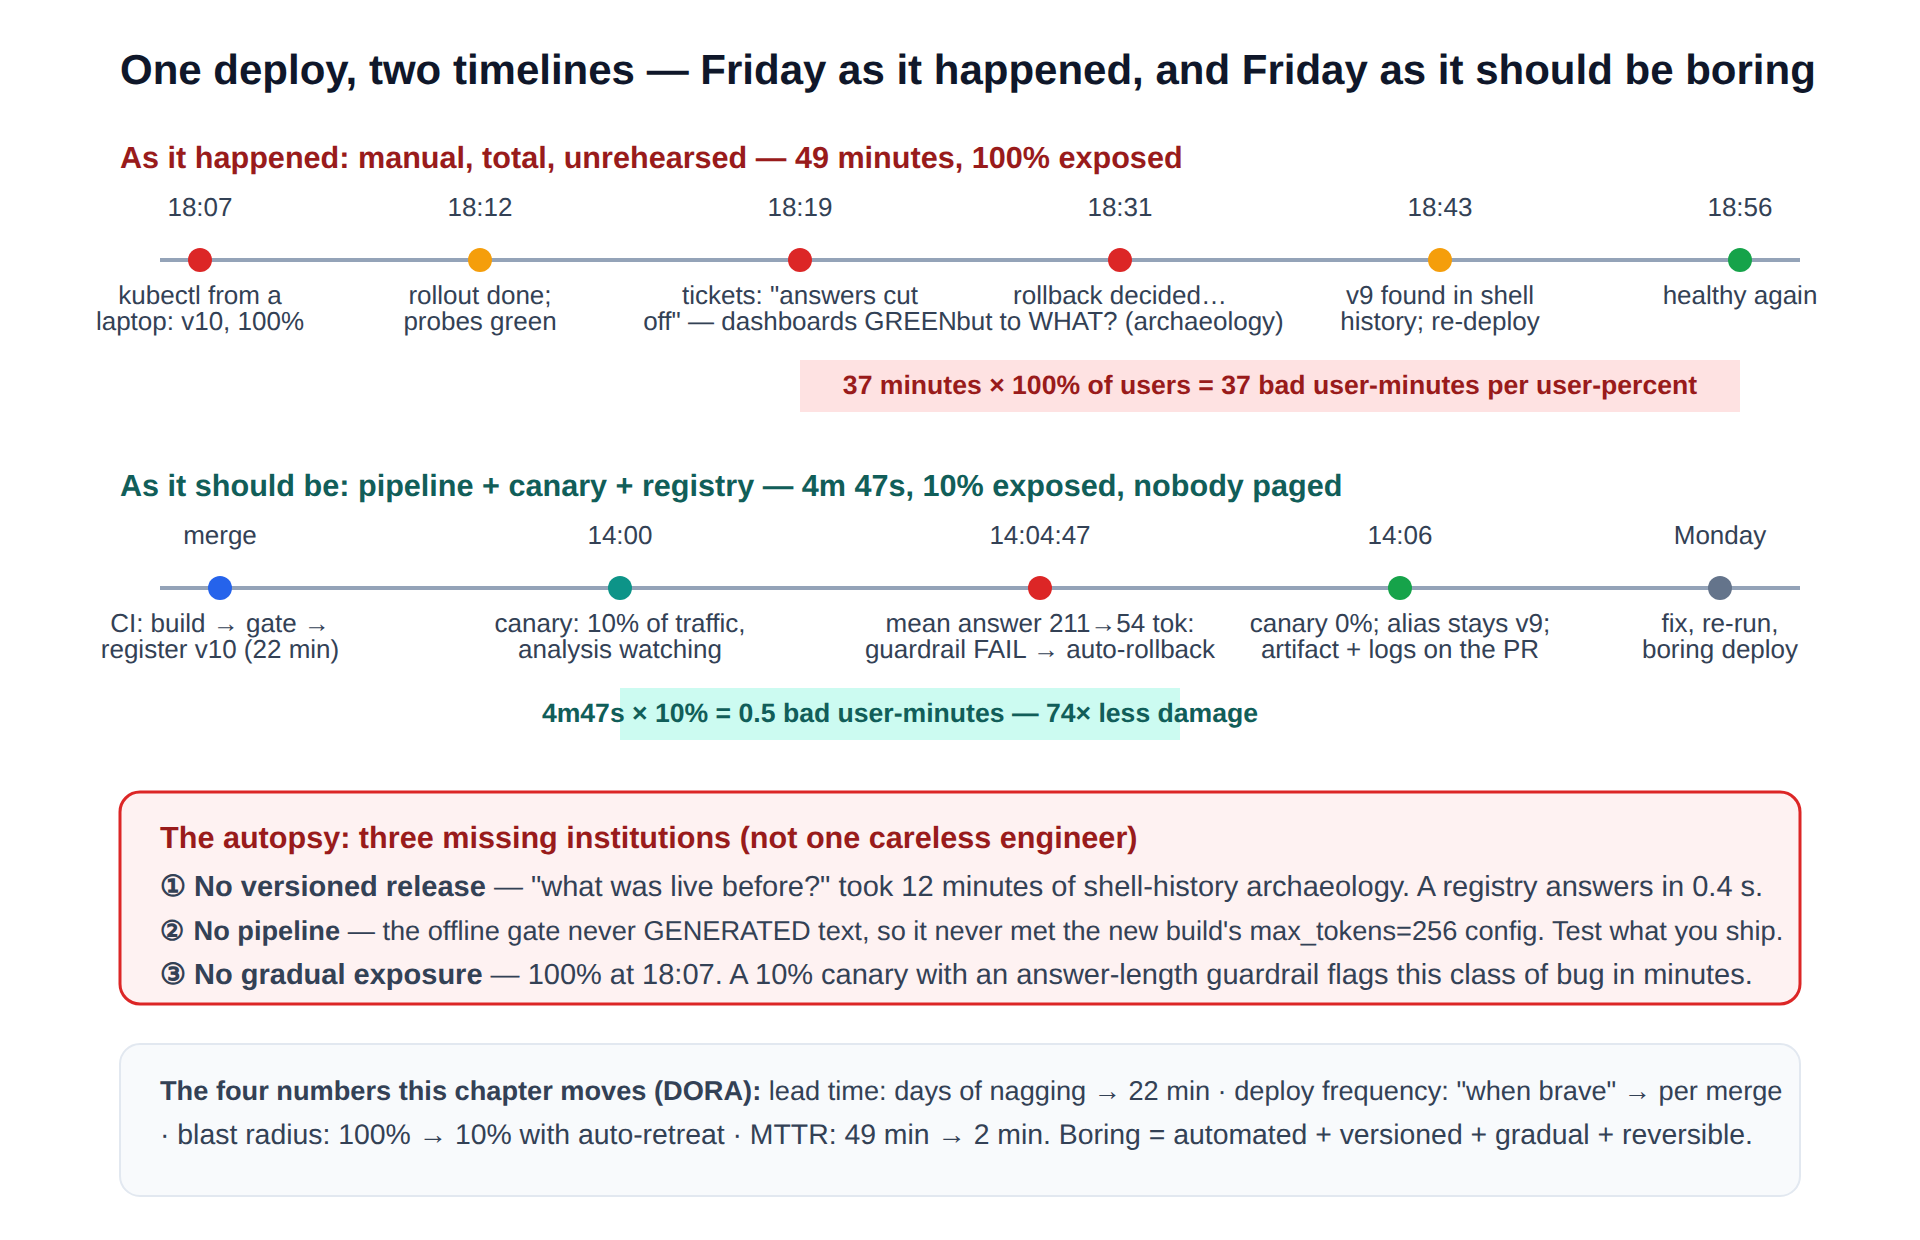
\includegraphics{figures/fig13-1_friday.png}}\\[3pt]
  \figcaption{Figure 13-1  One deploy, two timelines. Manual/total/unrehearsed: 49 minutes, all users. Pipeline/canary/registry: 4m47s, one user in ten, auto-retreat, evidence attached. The chapter is the distance between the two rows.}
\end{tbbfigure}

\subsection*{August 1, 2012: forty-five minutes, four hundred and sixty million dollars}

If Exhibit 13-A feels survivable — it was — industrial history supplies the version that was not, and it deserves two paragraphs because it is the canonical text of this chapter's discipline. \textbf{Knight Capital} was one of the largest market-makers in US equities: on a normal day its systems traded roughly one in every ten American shares. To meet an NYSE launch deadline, engineers manually deployed new order-routing code to the firm's \textbf{eight production servers... and missed one}. The new release reused an old feature flag — a flag that, on the un-updated eighth server, still pointed at \textbf{dead code from 2003}: a test module called Power Peg, designed to buy high and sell low on purpose (it existed to exercise other systems in a lab). When markets opened on August 1, 2012, the flag went live; seven servers ran the new code; the eighth woke the zombie. In \textbf{forty-five minutes} it fired millions of unintended orders across 154 stocks. Loss: about \textbf{\$460 million} — roughly \$170,000 per second — against a firm whose market value was \textasciitilde{}\$1 billion. The SEC's subsequent order is a catalog of this chapter's section headings stated as absences: no automated, verified deployment (a \textit{human} pushed to eight servers and no \textit{machine} confirmed eight of eight); no second review of the deploy; a reused flag binding new behavior to unversioned dead code; no kill switch; and — the detail that should stay with you — \textbf{while the system bled, nobody could say with confidence what was running where}, so the first "fix" (rolling back the \textit{new} code on the seven good servers, while the flag stayed on) made it \textit{worse}. Knight was effectively gone within the year, absorbed by a rival.

The industry's positive pole predates the disaster, which makes the contrast sharper. In 2009, two engineers from Flickr — John Allspaw and Paul Hammond — gave a conference talk with a title that sounded like a typo to most of the audience: \textbf{"10+ Deploys per Day."} Their claim, which seeded the entire DevOps movement, inverted the era's intuition that deploys are dangerous and should therefore be \textit{rare}: deploys are dangerous, they argued, and should therefore be \textbf{small, automated, observable, and constant} — a rare deploy is a large deploy, a large deploy is an unrehearsed high-stakes event, and an unrehearsed high-stakes event is Knight Capital. Fifteen years of industry measurement (the \textbf{DORA} research program) has since made the inversion quantitative: the teams that deploy \textit{most frequently} also have the \textit{lowest} change-failure rates and the fastest recovery — because frequency forces exactly the machinery this chapter builds. Four numbers summarize the target state, and Figure 13-1's bottom strip prices them for the course project: \textbf{lead time} from merge to production (days of nagging → a 22-minute pipeline), \textbf{deploy frequency} ("when someone is brave" → every merge), \textbf{change-failure blast radius} (100\% of users → a 10\% canary with automated retreat), and \textbf{time-to-restore} (49 minutes of archaeology → a 2-minute alias flip). The chapter's thesis in one sentence: \textbf{a deploy is boring precisely to the degree that it is automated, versioned, gradual, and reversible} — and boring is the highest compliment operations can pay.

The map for the ninety minutes ahead, each section one institution: \textbf{§13.2} builds the \textit{memory} — a registry over Chapter 6's store, where a release is a triple of digests with its gate report stapled on, promotion is an alias flip, and "what was live before?" is a 0.4-second query. \textbf{§13.3} builds the \textit{reflexes} — a GitHub Actions pipeline in three lanes that runs every gate this course has taught (Ch. 7's equivalence, Ch. 10's tolerance, Ch. 9's sweep) on every candidate, identically, and refuses loudly. \textbf{§13.4} builds the \textit{caution} — progressive delivery from rolling to canary to shadow, with the canary's automated analysis answering Chapter 12's dangling question: what does real traffic check that the gate cannot? \textbf{§13.5} looks over the fence at \textbf{managed endpoints} (SageMaker, Vertex), which sell most of this machinery as a service — same concepts, different YAML, plus a markup. And \textbf{§13.6} is the lab: build the pipeline, then earn the marks by \textit{failing to break production twice} — once at the gate, once at the canary. The deploy is boring; getting there is not.

\begin{calloutbox}{tbbpurple}{tbbpurplefill}
{\normalsize\bfseries\color{tbbpurple}Think About It}\par\vspace{3pt}
\begin{tbbitemize}
  \item Exhibit 13-A's dashboards stayed green through the whole incident — TTFT, TPOT, errors all fine. Using Chapters 7/11: WHY does the course's entire metric vocabulary miss this bug, and what is the smallest new metric that catches it? (You have just invented the guardrail metric — hold it for §13.4.)
  \item Knight's first responders rolled back the NEW code — and made it worse, because the real trigger was the reused FLAG on the eighth server. Restate the failure in this chapter's vocabulary (what was the "release"? what was versioned? what wasn't?), and name the §13.2 artifact that would have made "what is running where" a query instead of a guess.
  \item Steelman the opposite culture: a bank deploys its risk model quarterly, with a two-week review gate. Using DORA's logic, argue whether rare-and-heavy is EVER the right regime — and identify the hidden variable (batch size of change per deploy) that reconciles the bank with Flickr.
  \item Compute the bad-user-minutes for three worlds of Exhibit 13-A: (a) as it happened; (b) canary at 10\% with a 5-minute detection; (c) shadow mode (0\% exposure) that catches it pre-launch. What did each world COST in extra machinery — and which would you actually build first for the course project?
\end{tbbitemize}
\end{calloutbox}

\section{The Registry: Versions With Meaning}

Chapter 6 built a beautiful shelf and told you Week 13 would build the librarian. The store solved \textit{bytes}: immutable versions under clean prefixes, digests for identity, parallel loads, datasets and golden fixtures alongside. What it cannot do — structurally, as a pile of objects — is answer the only questions that matter at 2 a.m.: \textbf{which version is live? which is safe to roll back to? who checked this one, against what, and who approved it?} Friday's twelve minutes of archaeology were the price of asking a filesystem a governance question. A \textbf{model registry} is the database that answers: a small, boring, load-bearing catalog of \textit{promises about the bytes}. Its schema is worth learning as concepts rather than as any vendor's screens, because you will meet it wearing many logos (MLflow, Weights \& Biases, SageMaker's and Vertex's built-ins) and can build a serviceable one in an afternoon of JSON.

\begin{tbbfigure}
  \adjustbox{max width=0.94\linewidth,max totalheight=0.46\textheight}{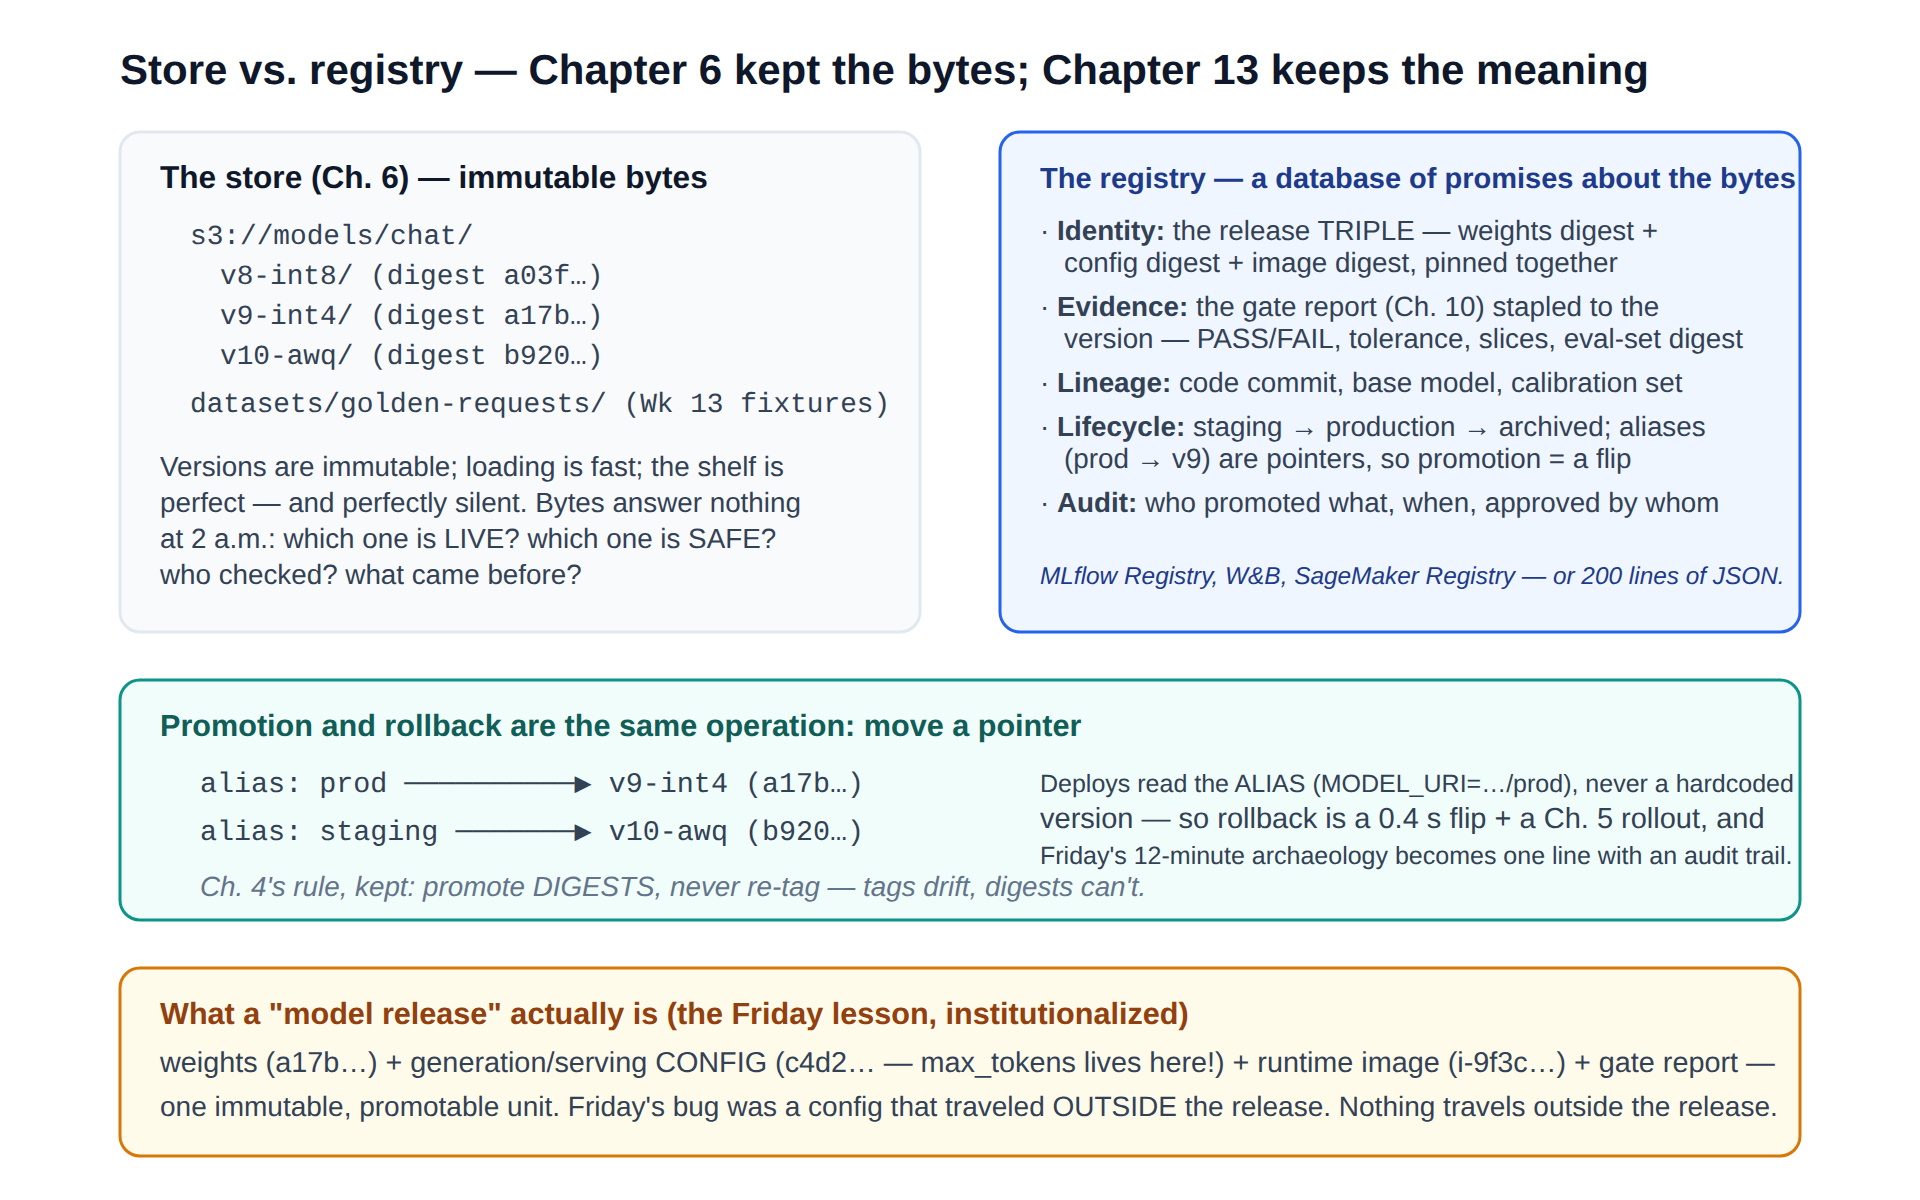
\includegraphics{figures/fig13-2_registry.png}}\\[3pt]
  \figcaption{Figure 13-2  Store vs. registry. The store keeps immutable bytes; the registry keeps identity (the release triple), evidence (the gate report), lineage, lifecycle (aliases), and audit. Promotion and rollback are the same operation: move a pointer.}
\end{tbbfigure}

\subsection*{The release triple — Friday's bug, made structurally impossible}

The registry's atom is not "a model." It is a \textbf{release}: the \textit{complete, immutable set of artifacts that answers requests together}. For this course's service that is a \textbf{triple of digests} — the weights (Ch. 6's prefix, digest \code{a17b…}), the serving/generation \textbf{config} (\code{c4d2…} — where max\_tokens, templates, sampling defaults live), and the runtime \textbf{image} (\code{i-9f3c…}, Ch. 4). Pin them together under one version number and Friday's failure class evaporates by construction: a config cannot "travel outside the release" because \textit{the release is defined as the thing that travels together}. Two disciplines make the atom trustworthy, both inherited. From Chapter 4: \textbf{promote digests, never re-tag} — that chapter's think-box asked why, and the answer is now visceral: a tag like \code{prod} that gets re-pushed is a name whose meaning changes under your feet (Knight's eighth server is what tag-drift looks like with money attached); a digest cannot drift. From Chapter 10: the \textbf{gate report is stapled to the version} — PASS/FAIL, the tolerance, the slice table, and the eval set's own digest — so "is v10 safe?" is a lookup, not a meeting.

\subsection*{Aliases: promotion as a pointer, rollback as a rehearsal}

The second idea is older than computing: \textbf{indirection}. Deployments never reference versions directly — Chapter 6's \code{MODEL\_URI} points at an \textbf{alias} (\code{…/\allowbreak chat/\allowbreak prod}), and the registry maps the alias to a version. Promotion is a pointer move (\code{prod: v9 → v10}); rollback is the same move backwards; both are atomic, logged, and take well under a second — the fleet then converges through the ordinary Chapter 5 rollout you have trusted since Week 5 (surge, probes, readiness gating), or merely re-resolves the alias on the next pod birth. Notice what this does to the 2 a.m. story: the \textit{decision} ("go back to v9") and the \textit{knowledge} ("v9 is the last version whose gate passed and which served production for 11 days") and the \textit{mechanism} (one command) now live in one place, rehearsed. The lab times this: \textbf{alias flip 0.4 s, fleet convergence \textasciitilde{}2 minutes} (§12.3's birth arithmetic — the rollback's floor is the cold start, which is why you rehearsed shrinking it). Lifecycle stages (staging → production → archived) are just distinguished aliases with rules attached: nothing reaches \code{production} without a gate report, an approval record, and — after §13.4 — a canary verdict.

\begin{terminalbox}
\begin{Verbatim}[breaklines=true,breakanywhere=true,fontsize=\small,formatcom=\color{tbbtermfg},codes=\tbbcodeactive]
$ python registry.py list chat
 ver  stage       weights        config   image     gate        by
 v8   archived    a03f…/int8     c11e…    i-77aa…   PASS 09-28  jslee
 v9   production  a17b…/int4     c4d2…    i-9f3c…   PASS 10-05  minj
 v10  staging     b920…/awq      c9aa…    i-2be1…   PASS 10-12  CI

$ python registry.py show chat/v10 --lineage
 commit 8d31f2  base Qwen2.5-3B  calib calib-2026-10a (digest 77e1…)
 eval-set golden-v4 (digest 3c9d…)  gate: delta -0.18pt (tol 0.5) PASS

$ python registry.py rollback chat --to v9        # the 2 a.m. one-liner
alias prod: v10 -> v9   (flip 0.4s; fleet converges via rollout)
audit: 2026-10-12T02:13Z rollback by oncall-kim, reason="ans-len"
\end{Verbatim}
\end{terminalbox}
\figcaption{Transcript 13-1  The registry, exercised. Three questions Friday could not answer — what is live, what is safe, what changed — each one line. The rollback is the same machinery as the promotion, which is why it can be rehearsed until boring.}

\subsection*{What bumps a version — the change taxonomy}

Teams stall on a deceptively small question: \textit{which changes deserve a new version?} The registry's answer is mechanical — \textbf{anything that changes any digest in the triple is a new release, full stop} — but the \textit{consequences} differ by change class, and writing them down once ends the recurring debate. Two subtleties earn their own sentences. \textbf{The config-only release} (Friday's fix: same weights, \code{max\_tokens} corrected) is a real release — new version, new gate run — but the gate can be \textit{scoped}: weights-identical means the equivalence battery is moot, while everything that touches generation (the golden requests, the guardrail baselines) must re-run, because config is precisely where Friday lived. \textbf{The eval-set change} is the sneaky one: it produces no release at all, yet it silently re-defines every future verdict — so eval sets version like code (golden-v4 → golden-v5, digest-pinned), old gate reports keep naming the set they ran against, and the first run after a set change \textit{re-baselines} rather than compares. A grade means nothing without knowing which exam.

\begin{tbbtablewrap}
  \begin{tabular}{@{}>{\raggedright\arraybackslash}m{\dimexpr 0.2500\tbltextwidth-2\tabcolsep\relax} >{\raggedright\arraybackslash}m{\dimexpr 0.2287\tbltextwidth-2\tabcolsep\relax} >{\raggedright\arraybackslash}m{\dimexpr 0.2660\tbltextwidth-2\tabcolsep\relax} >{\raggedright\arraybackslash}m{\dimexpr 0.2553\tbltextwidth-2\tabcolsep\relax}@{}}
  \arrayrulecolor{tbbnavy}\specialrule{1pt}{0pt}{0pt}
  \rowcolor{tbbtablehead}{\centering \bfseries\color{tbbnavy}Change} & {\centering \bfseries\color{tbbnavy}New release?} & {\centering \bfseries\color{tbbnavy}What re-runs} & {\centering \bfseries\color{tbbnavy}Typical strategy (§13.4)} \\
  \arrayrulecolor{tbbnavy}\specialrule{0.7pt}{0pt}{2pt}
  {\textbf{New weights (retrain/quant)}} & {Yes — new triple} & {Everything: equivalence, gate, sweep, canary} & {Canary; shadow at family boundaries} \\
  \arrayrulecolor{tbbtableborder}\hline
  {\textbf{Config only (sampling, tokens)}} & {Yes — config digest} & {Generation-path checks: golden requests, guardrail baselines, canary} & {Canary (Friday's class lives here!)} \\
  \arrayrulecolor{tbbtableborder}\hline
  {\textbf{Image only (deps, server code)}} & {Yes — image digest} & {Unit + golden requests + smoke sweep; gate skippable if weights/config identical} & {Rolling, canary if latency-relevant} \\
  \arrayrulecolor{tbbtableborder}\hline
  {\textbf{Eval set / golden fixtures}} & {No release — new SET version} & {Nothing ships; next gate re-baselines explicitly} & {— (a measurement change, not a deploy)} \\
  \arrayrulecolor{tbbtableborder}\hline
  {\textbf{Alias flip (promote/rollback)}} & {No — pointer move} & {Nothing: the referenced release was already checked} & {The 0.4 s operation itself} \\
  \arrayrulecolor{tbbnavy}\specialrule{1pt}{2pt}{0pt}
  \end{tabular}\par
  \figcaption{Table 13-1  The change taxonomy. The rule is one line — any digest change is a release — but knowing what re-runs keeps the pipeline fast and the debates short.}
\end{tbbtablewrap}

A word on build-vs-buy, since the concepts matter more than the logo. \textbf{MLflow's Model Registry} is the common open default (stages, aliases, lineage, a UI); the clouds bundle theirs; and the lab's \code{registry.py} is two hundred lines over a JSON file in the store — deliberately, so you see that the value is the \textit{schema and the discipline}, not the software. Whatever you adopt, hold it to the Friday test: from a cold terminal, can the on-call engineer answer \textit{live / safe / changed / who} in under a minute? If yes, it is a registry. If it needs a wiki page, it is a pile of bytes with opinions. For concreteness, here is the lab registry's entire schema — one entry, everything this section argued, in twenty lines of JSON that live (of course) in the store, versioned:

\begin{terminalbox}
\begin{Verbatim}[breaklines=true,breakanywhere=true,fontsize=\small,formatcom=\color{tbbtermfg},codes=\tbbcodeactive]
{ "model": "chat",
  "aliases": { "prod": "v9", "staging": "v10" },
  "versions": {
    "v10": {
      "triple": { "weights": "sha256:b920…", "config": "sha256:c9aa…",
                  "image":   "sha256:2be1…" },
      "gate":   { "verdict": "PASS", "delta_pt": -0.18, "tol": 0.5,
                  "worst_slice": ["streetcar", -0.6],
                  "eval_set": "golden-v4@sha256:3c9d…" },
      "lineage":{ "commit": "8d31f2", "base": "Qwen2.5-3B",
                  "calib": "calib-2026-10a@sha256:77e1…" },
      "history":[ {"t":"2026-10-12T09:14Z","event":"registered","by":"CI"},
                  {"t":"2026-10-12T14:03Z","event":"canary-retreat",
                   "by":"deploy.yaml","reason":"ans-len guardrail"} ]
  } } }
// promotion = edit "aliases" (atomically, via a conditional write).
// every field above is one 2 a.m. question, pre-answered.
\end{Verbatim}
\end{terminalbox}
\figcaption{Transcript 13-2  The registry-lite schema, whole. Triple, evidence, lineage, lifecycle, audit — the five ideas of this section as twenty lines of JSON. Vendors add UI and scale; the schema is the institution.}

\begin{calloutbox}{tbbpurple}{tbbpurplefill}
{\normalsize\bfseries\color{tbbpurple}Think About It}\par\vspace{3pt}
\begin{tbbitemize}
  \item Design the registry entry for a release that Friday's world could not even express: same weights as v9, NEW config (max\_tokens fix). What is its version? What does its lineage say? Why must it re-run the gate (which parts?) even though "the model didn't change"?
  \item Ch. 4 asked why pipelines promote digests rather than re-tagging. Answer it now with both failure stories at hand: the race (two engineers, one tag) and the rollback (what does "redeploy v9" mean if v9 was a tag someone re-pushed?). One paragraph each.
  \item Your PM asks: "MLflow is another service to run — why not a spreadsheet?" Grant the premise and find the breaking point: which registry property (atomic alias flips, audit, API for CI) dies first in a spreadsheet, and what incident does its death produce?
  \item The registry records who approved each promotion. Someone proposes auto-approving anything whose gate passes with 2× margin. Argue both sides using Exhibit 13-A (the gate was blind to the config) and §13.4's canary (which IS an automated approver) — where exactly does the human belong?
\end{tbbitemize}
\end{calloutbox}

\section{The Pipeline: Every Promise, Checked by a Machine}

The registry remembers; the \textbf{pipeline} enforces. Look back at what this course has actually accumulated since Week 7 and a remarkable fact appears: nearly every quality promise you have made is \textit{already executable}. The §7.6 equivalence battery is a script. The §10.3 gate is a script with a tolerance. The §9.5 sweep is a locustfile. The golden requests are files in the store (Ch. 6 planted them "for Week 13's CI gate"). What is missing is not checks but \textbf{ceremony}: a machine that runs all of them, in order, on every candidate, identically, with no way to skip the boring ones on a Friday. That machine is CI/CD — \textit{continuous integration} (every change is built and checked) flowing into \textit{continuous delivery} (every passing change is packaged, registered, and ready to promote). In Chapter 5's vocabulary, which is the correct one: the pipeline is just \textbf{one more writer of desired state} — it edits a registry alias and a Deployment env var, and the reconciliation loops do the rest. Nothing new runs in production; what is new is that nothing reaches production un-checked.

\begin{tbbfigure}
  \adjustbox{max width=0.94\linewidth,max totalheight=0.46\textheight}{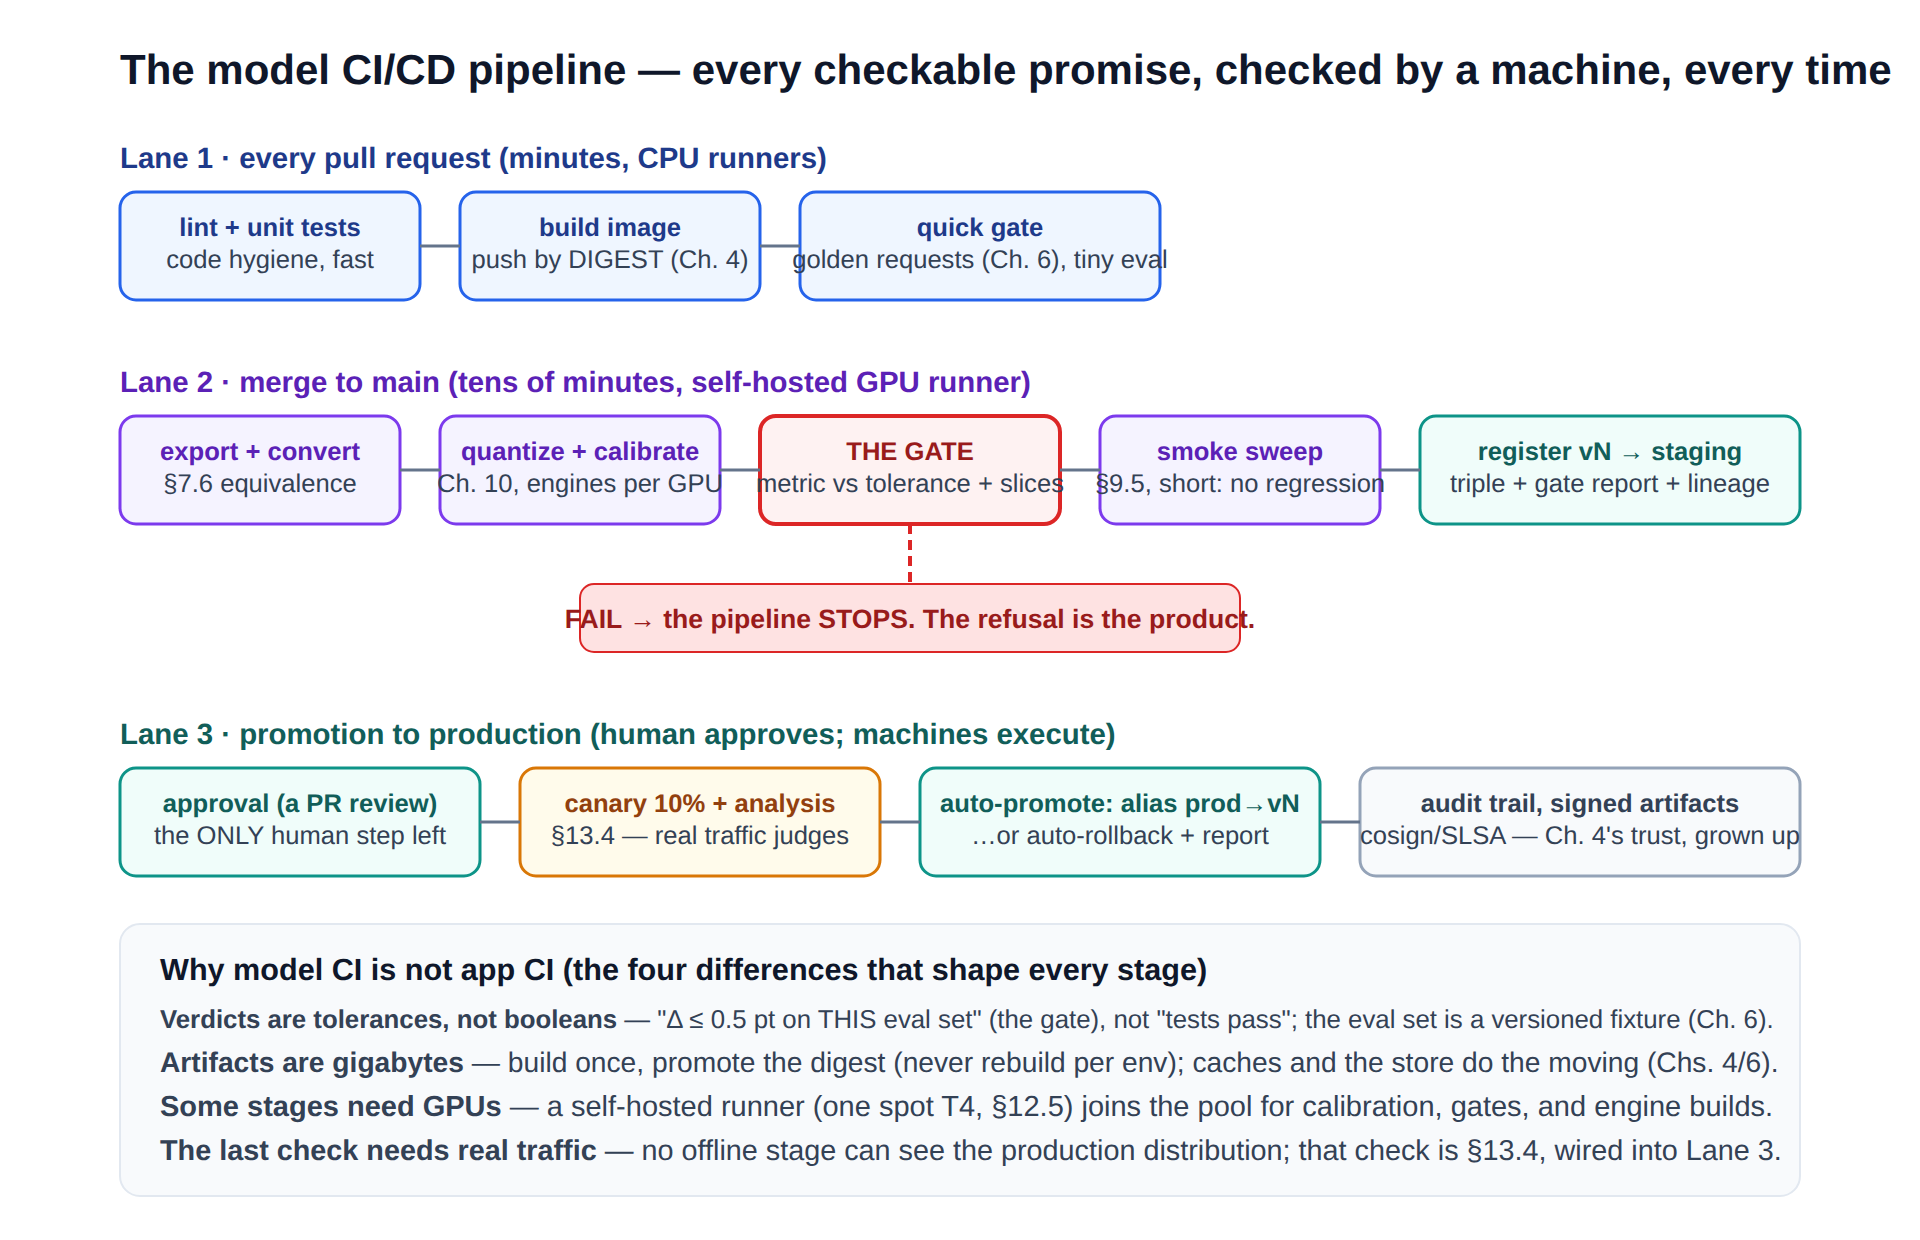
\includegraphics{figures/fig13-3_pipeline.png}}\\[3pt]
  \figcaption{Figure 13-3  Three lanes. Lane 1 (every PR): fast, CPU, hygiene. Lane 2 (every merge): the heavy artifacts and THE GATE, on a GPU runner — ending in a registered, evidence-bearing release. Lane 3 (promotion): a human approves; a canary judges; machines execute. The red path is the product.}
\end{tbbfigure}

\subsection*{Why model CI is not app CI — four differences that shape the design}

Teams that bolt a model onto an app pipeline discover four mismatches, and Figure 13-3's shape is the accommodation of each. \textbf{First, verdicts are tolerances on data, not booleans on code.} "Tests pass" becomes "Δ ≤ 0.5 pt top-1 \textit{on eval set golden-v4}" — which means the eval set is itself a versioned, digest-pinned fixture (change the exam and every historical grade silently changes meaning; Ch. 6 stored it for exactly this reason). \textbf{Second, artifacts are gigabytes.} App CI rebuilds cheaply per environment; model CI \textbf{builds once and promotes the digest} — the same bytes flow dev → staging → prod (Ch. 4's registries move only missing layers; Ch. 6's store moves nothing at all). Anything else re-introduces "works in staging" as a lie. \textbf{Third, some stages need silicon.} Calibration, gates, and engine builds want a GPU; GitHub's hosted runners don't have the right one, so a \textbf{self-hosted runner} — one spot T4 that registers itself with the repo (a 20-minute setup the handout scripts) — picks up the jobs tagged \code{gpu}. It is §12.5's portfolio thinking applied to CI: the runner is interruptible batch work, spot's true home. \textbf{Fourth, the final check needs real traffic} — no offline stage sees the production distribution, so the pipeline's last stage is not a test but a \textit{strategy}: §13.4's canary, wired in as Lane 3.

\begin{terminalbox}
\begin{Verbatim}[breaklines=true,breakanywhere=true,fontsize=\small,formatcom=\color{tbbtermfg},codes=\tbbcodeactive]
# .github/workflows/ci.yaml (condensed - the handout has the full file)
on:
  pull_request:                      # LANE 1: minutes, CPU
  push: {branches: [main]}          # LANE 2: the heavy lane
jobs:
  checks:                           # lane 1
    runs-on: ubuntu-latest
    steps: [lint, unit, docker build --push (by digest),
            quick-gate  # golden requests + 200-sample eval, CPU]
  release-candidate:                # lane 2
    if: github.ref == 'refs/heads/main'
    runs-on: [self-hosted, gpu]     # the spot T4 runner
    steps: [export + equivalence (§7.6),
            quantize + calibrate (Ch. 10),
            gate.py --tol 0.5       # FAIL -> the job fails. loudly.
            smoke-sweep (§9.5, 3 min),
            registry.py register --stage staging  # triple + report]
    permissions: {id-token: write}  # OIDC: no long-lived cloud keys
\end{Verbatim}
\end{terminalbox}
\figcaption{Transcript 13-3  The workflow, condensed. Lane 1 keeps PRs honest in minutes; lane 2 pays the heavy costs once per merge and ends in a registered release. The OIDC line is Ch. 4's auth question answered properly: the pipeline assumes a cloud role for minutes, and there is no key to leak.}

\subsection*{The two runs that matter — and the sentence that changes the team}

\begin{terminalbox}
\begin{Verbatim}[breaklines=true,breakanywhere=true,fontsize=\small,formatcom=\color{tbbtermfg},codes=\tbbcodeactive]
# run 1: merge 8d31f2 ("switch calib set to 2026-10a")   -- GREEN
  export+equivalence   PASS   max|dz|=3.1e-3, top1-agree 100%   4m
  quantize+calibrate   OK     awq int4, 1.91 GiB                 6m
  gate                 PASS   delta -0.18pt (tol 0.5);
                              worst slice "streetcar" -0.6pt     7m
  smoke sweep          PASS   468 tok/s agg (-2.1% vs base)      3m
  register             OK     chat/v10 -> staging (evidence attached)
  total 22m 14s        bot comment on PR: report + artifact links

# run 2: merge a90c11 ("improve prompt template")        -- RED
  quick-gate           FAIL   golden request 07: expected JSON,
                              got prose; 09: missing citation;
                              12: language mismatch (ko->en)     1m31s
  >> merge blocked. no build, no registry entry, no debate.
# the check that refused has passed 41 times. it is not an opinion.
\end{Verbatim}
\end{terminalbox}
\figcaption{Transcript 13-4  The two runs that matter. Green is pleasant bureaucracy ending in an evidence-bearing registry entry. Red is the institution: ninety-one seconds, three named regressions, a greyed-out merge button — and a quality dispute that never became an argument.}

The red run is the purchase, and the cultural mechanics deserve one paragraph. When the quick gate catches the prompt-template regression, \textit{the merge button greys out} — and \textbf{nobody argues with it}, because the check that refused is the same check that has passed forty-one times, not a colleague with an opinion. The pipeline converts quality disputes from interpersonal to infrastructural. Two disciplines keep that credibility. \textbf{Never skip, never fork}: the moment a \code{[skip-gate]} commit tag exists, Friday exists again — the emergency path is a \textit{faster canary}, not a skipped gate. \textbf{The pipeline eats its own artifacts}: what was gated is byte-identically what deploys (digests, again); any re-build between check and ship un-checks everything. And a supply-chain note the security team will eventually send anyway: signing artifacts (cosign) and recording provenance (SLSA) — Chapter 4's "trust the digest" grown up — belongs in Lane 2 from the start; it is two steps in the workflow now and an archaeology project later.

One security paragraph the lab enforces, because the mistake is common enough to have its own incident genre. A \textbf{self-hosted runner executes whatever the workflow tells it to} — which means a runner attached to a \textit{public} repo, triggered by \textit{fork} pull requests, is an arbitrary-code-execution service with your GPU, your network position, and (if you were careless) your cloud credentials. The disciplines: self-hosted runners serve \textbf{private repos or non-fork triggers only} (Lane 1's fork-facing checks stay on GitHub's hosted runners); the runner's cloud role is scoped to exactly its jobs (the OIDC trust policy names the repo and branch); and treat \code{pull\_request\_target} as the foot-gun the docs say it is. None of this is exotic — it is Chapter 2's isolation instinct applied to the machine that builds the thing that runs in production, which makes it \textit{more} sensitive than production, not less: compromise the pipeline and every future green check is a lie.

\begin{calloutbox}{tbbpurple}{tbbpurplefill}
{\normalsize\bfseries\color{tbbpurple}Think About It}\par\vspace{3pt}
\begin{tbbitemize}
  \item Your quick gate (Lane 1) uses 200 eval samples for speed; the full gate (Lane 2) uses 10,000. Compute the statistical price: if the true regression is 1.0 pt, roughly what Δ can each detect reliably (rule of thumb: noise ≈ 1/√n)? What class of bug does Lane 1 therefore EXIST to catch, if not accuracy drift?
  \item The self-hosted GPU runner is a spot instance. Walk the failure: it gets reclaimed mid-gate. What does the workflow show? What must the job be for this to be merely annoying (idempotent stages, resumable artifacts) — and why is a CI runner spot's truest home (§12.5's language)?
  \item A teammate proposes gating on the SWEEP (throughput) with a hard threshold: "reject if req/s@SLO drops >5\%." Defend and attack: what infrastructure noise (Ch. 9) makes a hard throughput gate flaky, and what two-tier design (warn vs. block; relative-to-rebaseline) keeps the signal without the 2 a.m. false alarms?
  \item Write the team's emergency-deploy policy in three sentences, given "never skip the gate" — what DOES change in an emergency (canary speed? approval quorum? rollback pre-staging?), and what never does? Then check it against Knight: would your policy have saved them?
\end{tbbitemize}
\end{calloutbox}

\section{Meeting Real Traffic: Rolling, Blue/Green, Canary, A/B, Shadow}

The pipeline's last stage cannot be a test, because the thing it must check does not exist offline: \textbf{production traffic}. Your eval sets are a rear-view mirror of last month's users; your staging cluster is a diorama; the true distribution — tonight's slang, this morning's outage-driven panic queries, the whale who pastes 30k-token contracts — exists in exactly one place. Every strategy in this section is a different protocol for letting a new release \textit{meet reality} with a hand on its collar, and the crucial discipline is that they answer \textbf{different questions}. Choose by question, not by fashion: rolling asks \textit{does it boot?}; blue/green asks \textit{can I undo in one second?}; canary asks \textit{is it broken, judged by real traffic?}; A/B asks \textit{is it better, judged by users?}; shadow asks \textit{what would it have done?} — before anyone risks anything at all.

\begin{tbbfigure}
  \adjustbox{max width=0.94\linewidth,max totalheight=0.46\textheight}{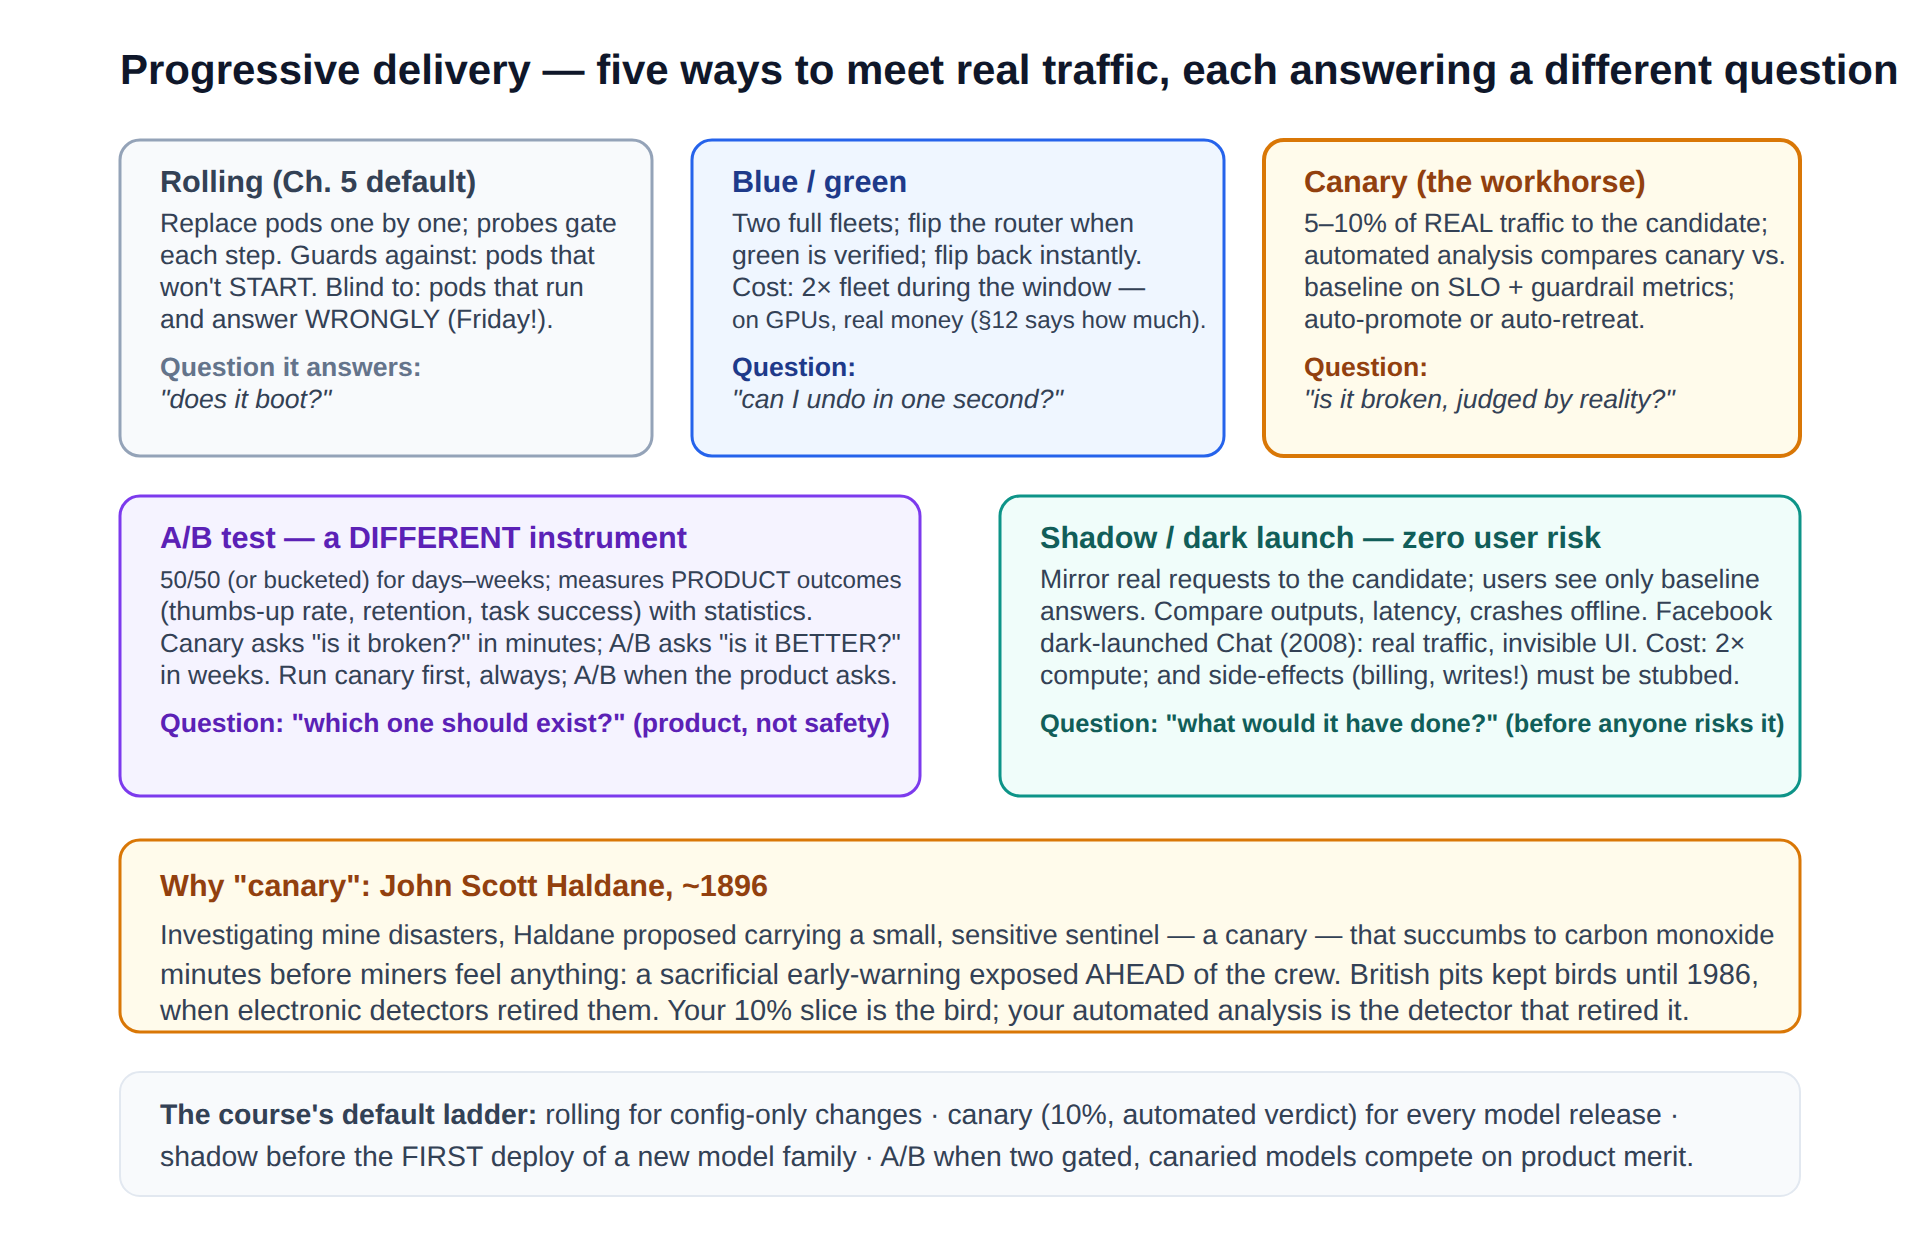
\includegraphics{figures/fig13-4_strategies.png}}\\[3pt]
  \figcaption{Figure 13-4  Five strategies, five questions. Rolling guards startup; blue/green buys instant undo at 2× fleet; the canary is the workhorse verdict on real traffic; A/B is a product instrument, not a safety one; shadow rehearses with zero user risk. Bottom: Haldane's birds, and the detector that retired them.}
\end{tbbfigure}

\subsection*{Rolling and blue/green — the inherited rungs}

\textbf{Rolling} you have owned since Chapter 5: replace pods a few at a time, each admitted by its readiness probe. Understand precisely what it guards — \textit{pods that fail to start or fail their probe} — and what it is blind to: Friday's pod started beautifully, probed warm, and served short answers with perfect health. Rolling is the right whole strategy only for changes whose failure mode IS startup (dependency bumps, resource tweaks); for model releases it is the \textit{substrate} the smarter strategies ride on. \textbf{Blue/green} runs two full fleets — blue serving, green idle with the candidate — verifies green (smoke tests, warm caches), then flips the router; regret is a flip back, seconds, total. Its honesty problem on GPU fleets is Chapter 12's arithmetic: a second fleet is a second bill (\textasciitilde{}\$1,500/mo for the course fleet during every release window — tolerable for minutes, obscene as a habit), and the pre-flip verification is still \textit{synthetic} traffic, so it shares rolling's blindness to Friday-class bugs. Where blue/green shines is the \textit{config/infra} release with instant-undo requirements (engine upgrades, CUDA bumps) — and its router-flip mechanism is, not coincidentally, exactly the muscle the canary reuses at finer grain.

\subsection*{The canary — Haldane's bird, and the detector that retired it}

The workhorse deserves its etymology, because the metaphor is load-bearing. Investigating mine explosions in the 1890s, the physiologist \textbf{John Scott Haldane} proposed that crews carry a small, warm-blooded sentinel — a canary — whose faster metabolism made it succumb to carbon monoxide \textit{minutes before miners felt anything}: a sensitive, sacrificial detector exposed \textbf{ahead of the crew}, cheap to watch (the bird stops singing, then sways) and cheap to act on (walk out). British pits carried birds until \textbf{1986}, when electronic detectors finally retired them. Map every clause: the \textbf{canary release} takes 5–10\% of real traffic (the bird breathes the real air) while 90\% stays on the incumbent (the crew waits at the entrance); an \textbf{automated analysis} watches it (the electronic detector — your upgrade over 1911: nobody has to remember to look at the bird); and a bad verdict triggers \textbf{auto-retreat} in seconds (walking out). Three design choices make or break it in this course's domain. \textit{Split by session, not by request} — a Chapter 11 conversation must live wholly on one side (consistent-hash on conversation id, §11.5's affinity machinery moonlighting), or users see personality flicker and your metrics compare mush. \textit{Judge canary against baseline, concurrently} — never against yesterday: the traffic itself has a diurnal personality (Ch. 12), and only a same-time control isolates the release. \textit{Watch guardrails, not just SLOs} — and here the Friday bug pays its tuition.

\begin{tbbfigure}
  \adjustbox{max width=0.94\linewidth,max totalheight=0.46\textheight}{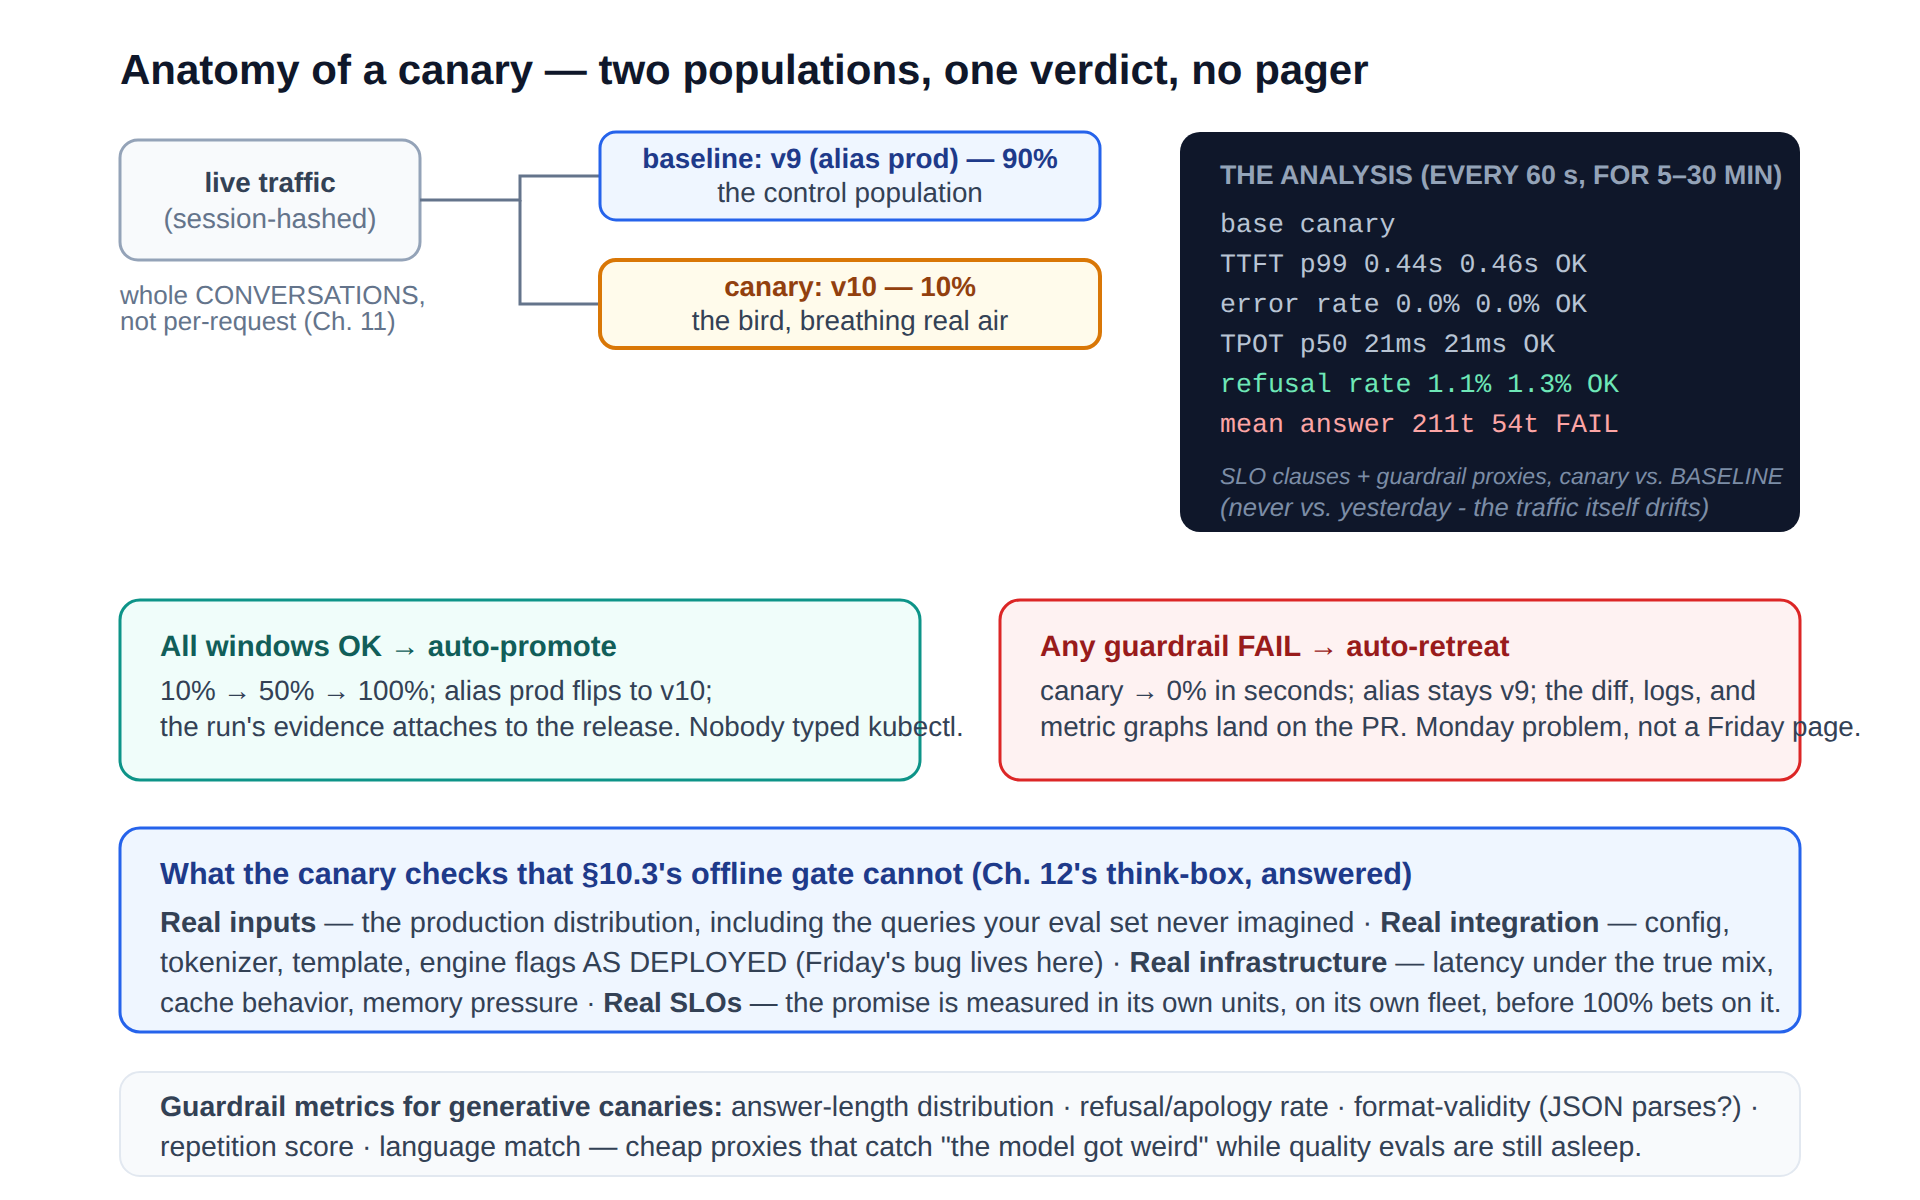
\includegraphics{figures/fig13-5_canary.png}}\\[3pt]
  \figcaption{Figure 13-5  The canary's anatomy: session-hashed split, concurrent baseline, a 60-second analysis loop over SLO clauses plus guardrail proxies, and two automatic exits. The FAIL row is Friday's bug, caught at 10\% in under five minutes.}
\end{tbbfigure}

\textbf{Guardrail metrics} are the generative era's addition to canary lore, and your §13.1 think-box already invented them: cheap, model-agnostic proxies that catch \textit{"the model got weird"} while true quality evals are still asleep. The course set, all computable from logs in a 60-second loop: \textbf{answer-length distribution} (Friday's 211 → 54 tokens screams in one window), \textbf{refusal/apology rate} (over-alignment regressions), \textbf{format validity} (does the JSON parse? do citations resolve?), \textbf{repetition score}, \textbf{language match} (Korean question → Korean answer). None measures "goodness"; all measure \textit{sameness of behavior}, which is precisely a deploy's null hypothesis — the SLO clauses (TTFT/TPOT/error, Ch. 11) guard the system, the guardrails guard the \textit{behavior}, and anything subtler waits for A/B. The verdict logic stays deliberately dumb: fixed windows, explicit thresholds vs. baseline, ANY failure → retreat. (Tools: Argo Rollouts — Chapter 5's further reading, arrived — automates step-weights and analysis against Prometheus for raw Deployments; KServe's \code{canaryTrafficPercent}, Chapter 12's dangling knob, does it for InferenceServices; the lab drives the latter with a 40-line loop so you see there is no magic.)

\begin{terminalbox}
\begin{Verbatim}[breaklines=true,breakanywhere=true,fontsize=\small,formatcom=\color{tbbtermfg},codes=\tbbcodeactive]
$ gh workflow run deploy.yaml -f version=v10      # lane 3, replayed
14:00:12  canary: chat canaryTrafficPercent 0 -> 10 (session-hashed)
14:01:12  window 1/5:  TTFT p99 0.46s vs 0.44s OK | err 0.0% OK
          | ans-len 208t vs 211t OK | refusal 1.2% vs 1.1% OK
14:02:12  window 2/5:  all OK
14:03:12  window 3/5:  ans-len 55t vs 210t
          guardrail: |delta| 74% > 30%  -> FAIL
14:03:14  verdict: RETREAT. canary 10% -> 0%. alias prod stays v9.
14:03:20  posted to PR #241: verdict, metric graphs, sample diffs
          (12 canary answers, all ending mid-sentence at 54 tokens)
# exposure: ~10% of users for 3m02s = 0.3 bad user-minutes.
# friday, replayed with institutions: the bird went quiet,
# the detector noticed, the crew never entered the mine.
\end{Verbatim}
\end{terminalbox}
\figcaption{Transcript 13-5  The Friday bug vs. the canary. Three windows, one tripped guardrail, automatic retreat, evidence filed where the fix will happen. Nobody was paged, because nothing needed a human — the entire incident is a PR comment.}

\subsection*{How long is long enough — the canary's statistics, on a napkin}

The window length is not folklore; it is sample-size arithmetic you can do in your head. The course fleet at peak absorbs \textasciitilde{}23 turn-arrivals/s (§11.2), so a 10\% canary sees \textbf{\textasciitilde{}2.3 requests/s ≈ 690 answers in five minutes} — and what 690 samples can detect depends entirely on the effect's size. Friday's cliff (answer length 211 → 54 tokens, a 74\% drop against a distribution whose spread is \textasciitilde{}±30\%) is unmistakable within the \textit{first} 60-second window — cliffs need dozens of samples, which is why Transcript 13-5's verdict lands in window three with margin to spare. But a \textit{subtle} regression — say a 3\% dip in format-validity from 97\% — needs on the order of thousands of samples per arm to separate from noise (binomial rule of thumb: detectable Δ ≈ 2√(p(1−p)/n) — at n = 690, roughly ±1.3 percentage points at best). Hence the design stance worth memorizing: \textbf{canaries catch cliffs, not slopes.} Configure them for the cliff classes (crashes, SLO breaks, guardrail jumps) with short dwell and hard thresholds; leave slopes to the instruments built for them — Chapter 14's drift monitors (weeks of production data) and §13.4's A/B (balanced arms, pre-registered power). The step-up schedule encodes the same logic as exposure control: 1\% → 10\% → 50\% → 100\% with a dwell per step means the cheapest cliffs are caught at 1\% (crashes need \textasciitilde{}ten samples), the guardrail cliffs at 10\%, and the long tail of "we'll see" is bounded by the final dwell — each step buys detection power with user exposure, and writing the schedule down turns a judgment call into a config field.

\subsection*{A/B and shadow — the other two questions}

\textbf{A/B testing} shares the canary's traffic-splitting plumbing and \textit{nothing else} — confusing them is the section's classic error. The canary is a \textbf{safety} instrument: minutes-to-hours, small exposure, null hypothesis "behaves the same," verdict automatic. A/B is a \textbf{product} instrument: days-to-weeks, large balanced buckets (often 50/50), hypothesis "v10's answers are \textit{better}," measured in product outcomes (thumbs-up rate, task completion, retention) with actual statistics — pre-registered metrics, power analysis, novelty-effect patience. For LLM products A/B is where quality claims go to be tested honestly (win-rate on real sessions beats any offline benchmark), but it \textit{presumes} the candidate already passed gate and canary: you A/B two safe models to learn which should exist, never to discover whether one is broken. \textbf{Shadow (dark launch)} completes the spectrum at zero user risk: mirror a copy of real traffic to the candidate, users see only the incumbent's answers, and you diff the shadow's behavior offline — crashes, latency under the true mix, output drift, all before exposure. Facebook's famous 2008 \textbf{dark launch} of Chat did this at scale: for weeks, pages silently opened connections and simulated the message path with real traffic shapes, no UI — the launch-day load was old news to the backend. The costs are real: \textasciitilde{}2× inference compute for the mirrored slice (Ch. 12 prices it — shadow 10\% of traffic ≈ one extra replica-hour per ten), and \textbf{side-effects must be stubbed} (a shadow that writes to billing, sends emails, or mutates the KV of a shared cache is not a rehearsal, it is a second production). Shadow earns its cost at \textit{family boundaries} — the first vLLM deploy, a new base model, an engine major-version — where the canary's 10\% is still 10\% of real users on genuinely unknown behavior.

The course's default ladder, then, one line per rung (Figure 13-4's bottom strip): \textbf{rolling} alone for code/config changes whose failure is startup-shaped; \textbf{canary with automated analysis} for \textit{every} model release, no exceptions — it is the cheapest institution per bad-user-minute saved in this entire course; \textbf{shadow first} when the release crosses a family boundary; \textbf{A/B} when two gated, canaried candidates compete on merit. And the meta-rule that makes the ladder work under pressure: \textbf{the strategies are pipeline stages, not heroic choices} — Lane 3 runs the same YAML whether it is Tuesday afternoon or Friday 18:07, which is the entire point.

\begin{calloutbox}{tbbpurple}{tbbpurplefill}
{\normalsize\bfseries\color{tbbpurple}Think About It}\par\vspace{3pt}
\begin{tbbitemize}
  \item The canary passed but users are complaining a week later. List three failure classes a 30-minute canary structurally CANNOT catch (slow-burn quality drift, low-frequency slices, novelty effects) — and for each, name the §13.4 or Ch. 14 instrument that does.
  \item Session-hashing sends 10\% of CONVERSATIONS to the canary. A power user with 200 conversations/day complains they "always get the weird one." Compute their odds under per-session vs. per-user hashing, and redesign the split key — what does your fix cost the analysis (sample independence)?
  \item Design the shadow harness for the course project in detail: where does traffic fork (LB? sidecar? async tap from logs?), what is stubbed, what is diffed, and what is the ONE number that decides "ready for canary"? Include the §12 cost line.
  \item Your PM wants to skip canary for a "tiny prompt tweak." Using Exhibit 13-A (a "tiny config" change), the guardrail table, and the cost of a canary (≈zero marginal — the pipeline runs it anyway), write the two-sentence reply — then name the ONE change class where skipping canary is actually defensible (hint: §13.4's first rung).
\end{tbbitemize}
\end{calloutbox}

\section{Managed Endpoints: The Operator Ladder, Completed}

Everything this chapter built, someone will sell you. \textbf{SageMaker endpoints} (AWS) and \textbf{Vertex AI endpoints} (GCP) — with kin at every cloud — are the final rung of the operator ladder Chapter 12 started: DIY (you run everything) → platform (KServe's operator runs the serving plumbing on \textit{your} cluster) → \textbf{managed} (their operator, their cluster, their pager). Upload a model artifact, choose an instance type, and the vendor conjures what Chapters 5–12 taught you to build: provisioning, autoscaling, health-based routing, logging, patching — plus, germane to this chapter, \textbf{production variants / traffic splits} (canary as a field: SageMaker's \code{InitialVariantWeight}, Vertex's \code{trafficSplit \{v9: 90, v10: 10\}}), \textbf{model registries} with approval workflows, and \textbf{deployment guardrails} (auto-rollback on alarm — §13.4's analysis, sold as a checkbox). The vocabulary maps one-to-one, which is exactly why this section is short: you already know what every knob does, because you built the knob.

\begin{tbbfigure}
  \adjustbox{max width=0.94\linewidth,max totalheight=0.46\textheight}{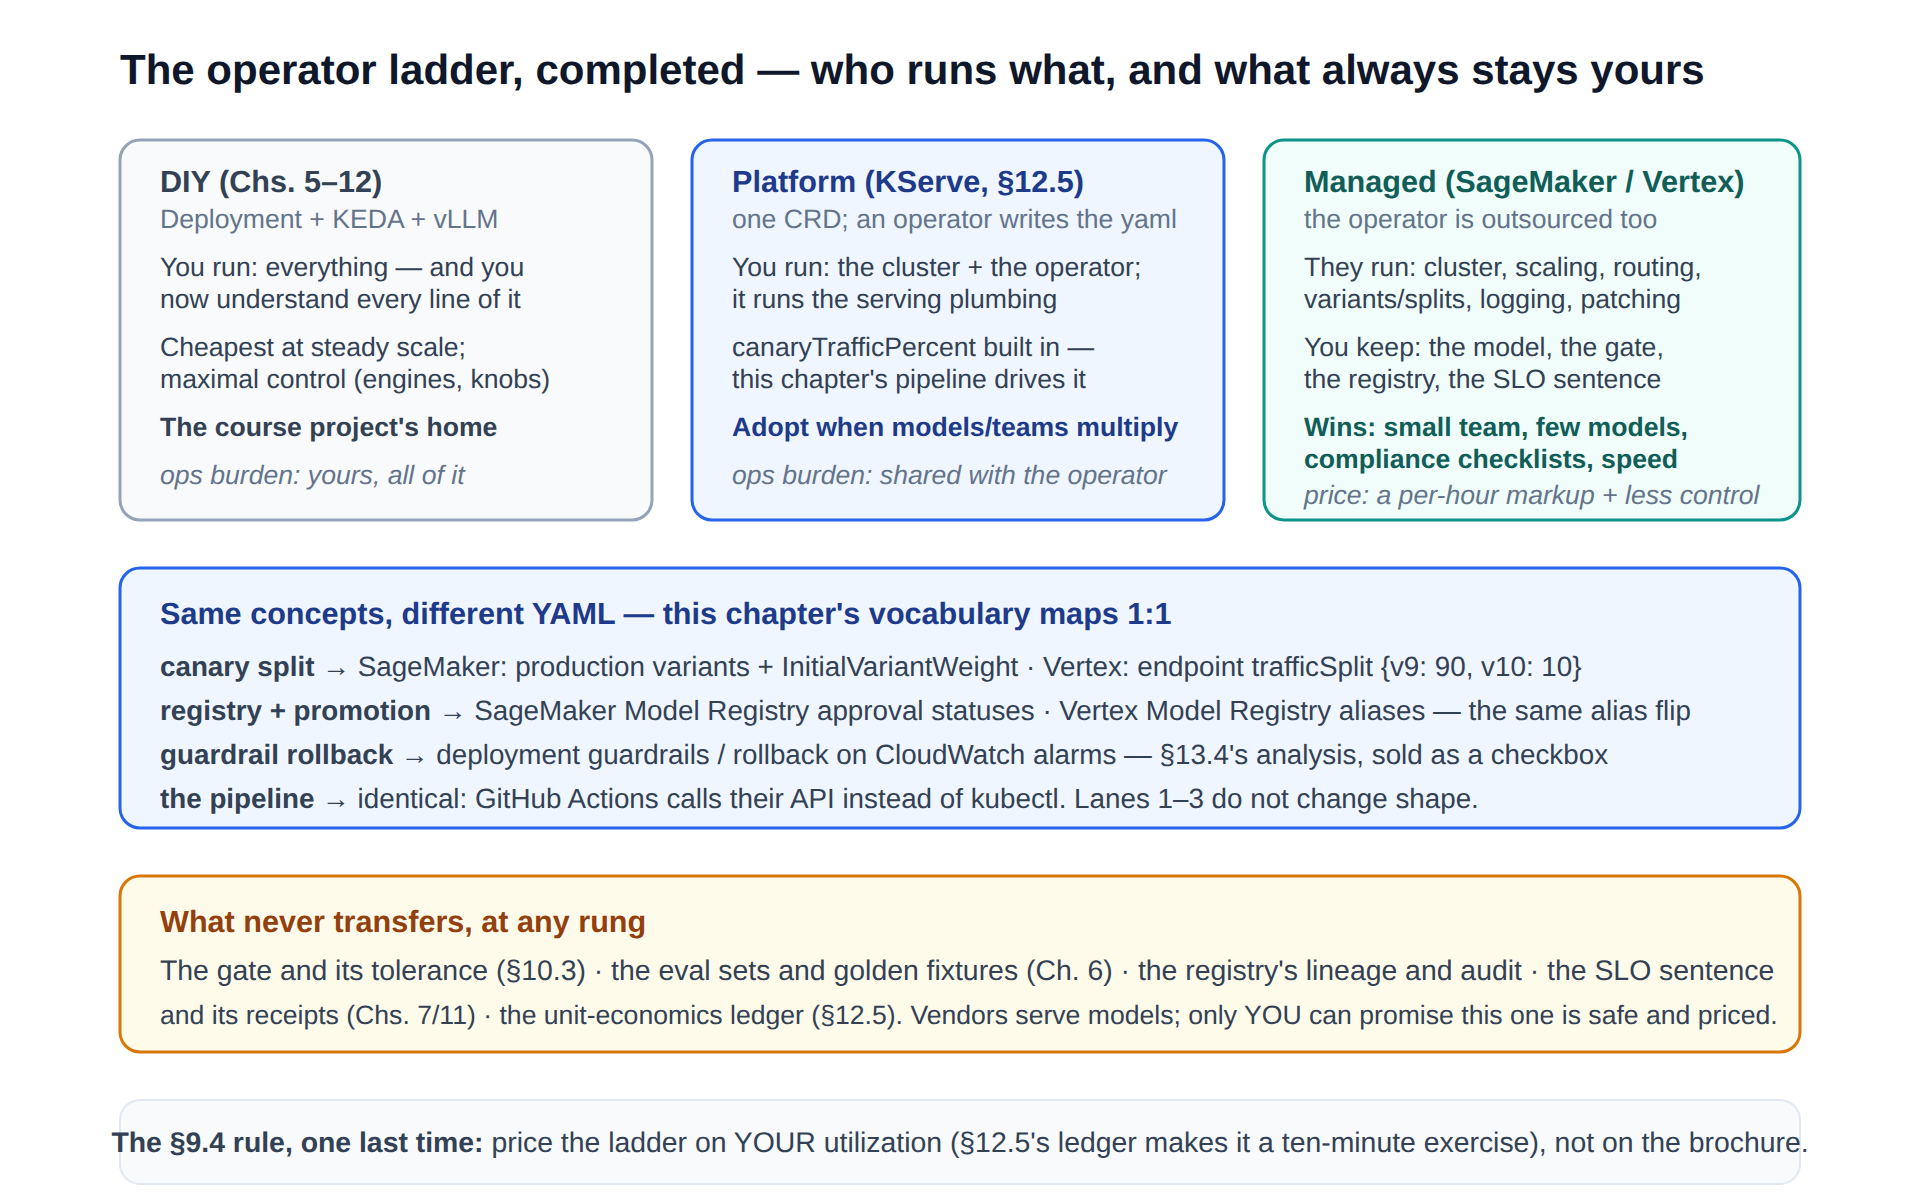
\includegraphics{figures/fig13-6_managed.png}}\\[3pt]
  \figcaption{Figure 13-6  The ladder's last rung. Managed endpoints run the plumbing and sell this chapter's strategies as fields — while the gate, the eval sets, the registry's lineage, the SLO sentence, and the unit-economics ledger remain yours at every rung, forever.}
\end{tbbfigure}

The honest trade, priced with tools you now own. \textbf{What you get}: a team of zero runs a production model this afternoon; compliance checklists inherit the vendor's certifications; the undifferentiated heavy lifting (node pools, drivers, CVE patching, §12.3's cold-start engineering) becomes someone else's Q3. \textbf{What you pay}: a per-instance-hour \textbf{markup} over raw VMs (routinely tens of percent — run §12.5's ledger against your utilization before believing either direction), less control over the serving stack (engine versions, §9/§11 knobs, custom kernels arrive on the vendor's schedule), their cold-start and scale-to-zero policies rather than yours, and gravity (egress, IAM webs, retraining muscles atrophy). The decision is Chapter 9's benchmark rule wearing a suit: \textit{price the ladder on your utilization and your team, not on the brochure} — small team + few models + spiky traffic leans managed; steady scale + cost pressure + engine-level tuning (this course's project, by design) leans down-ladder. And one asset never transfers, at any rung: \textbf{the gate and its tolerance, the eval fixtures, the registry's lineage and audit, the SLO sentence with receipts, the \$/M-token ledger} — vendors serve models; only you can promise that \textit{this} one is safe, priced, and honestly measured. That list, you may notice, is simply this course.

Because "run the ledger" deserves to be shown once rather than assigned, here is the course fleet re-priced on the managed rung, with §12.5's own arithmetic. Assume a representative \textbf{35\% markup} on the L4-class instance and the vendor's autoscaling honoring the same 61 rep-h/day staircase (their scale-to-zero policies rarely beat your floor-of-2 reasoning, so keep it). Compute: 61 × 31 × (\$0.80 × 1.35) ≈ \textbf{\$2,042/mo} against the self-hosted \$1,513 — a \$529/mo premium — and the managed rung takes commitments but \textit{not} your spot-burst trick, so the realistic gap widens toward \textbf{\textasciitilde{}\$1,100/mo vs. \$877}. What the premium buys, priced in the only honest unit: roughly \textbf{one engineer-week per quarter} of not building §12.2–12.3, §13.4-as-checkbox, and the patching treadmill. For a two-person team with three models, that trade is frequently \textit{correct}; for this course's project — one hot model, engine-level tuning, a team that now owns every knob — it is not. The point is not the verdict; it is that the verdict took four lines of arithmetic and zero brochures, which is what fourteen weeks of measured numbers are \textit{for}.

\begin{calloutbox}{tbbpurple}{tbbpurplefill}
{\normalsize\bfseries\color{tbbpurple}Think About It}\par\vspace{3pt}
\begin{tbbitemize}
  \item Rebuild Transcript 12-6's ledger for a managed endpoint at a 35\% instance markup with scale-to-zero on the long tail included. At what fleet size does the markup exceed one SRE-month per year — and why is THAT the actual break-even question, not the GPU price?
  \item A regulated customer requires "no shared infrastructure below the hypervisor." Walk each ladder rung against the requirement using Chapter 2's isolation vocabulary (passthrough, MIG, multi-tenant control planes) — which rungs survive, and what do the survivors cost?
  \item Your pipeline (Lanes 1–3) targets kubectl today. Enumerate exactly which steps change if the deploy target becomes a Vertex endpoint (hint: only Lane 3's verbs) — and which artifacts (triple, gate report, registry entry) must NOT change, on pain of un-checking what was checked.
  \item Managed guardrails auto-rollback on CloudWatch alarms — infrastructure metrics. Using Friday's bug, explain the gap between vendor guardrails and §13.4's guardrail METRICS, and design the smallest lambda/cloud-function that closes it (what does it read, compute, and call?).
\end{tbbitemize}
\end{calloutbox}

\section{Lab: Build the Pipeline, Then Fail to Break Production}

The syllabus names the deliverable — \textbf{GitHub Actions로 모델 자동 배포 파이프라인 구축} — and this lab takes its grading philosophy from §13.3: a pipeline is proven by what it \textit{refuses}. You will wire the three lanes onto your project repo from a handout skeleton, produce one green path end to end, and then earn the majority of the marks by attacking your own production \textbf{twice and failing twice} — once at the gate, once at the canary. Budget: \textasciitilde{}\$2 of GPU-runner time; the T4 does double duty as the self-hosted runner and the serving node. Teams on the CPU fallback path run every stage with the small model — the pipeline neither knows nor cares, which is rather the point.

\begin{tbbfigure}
  \adjustbox{max width=0.94\linewidth,max totalheight=0.46\textheight}{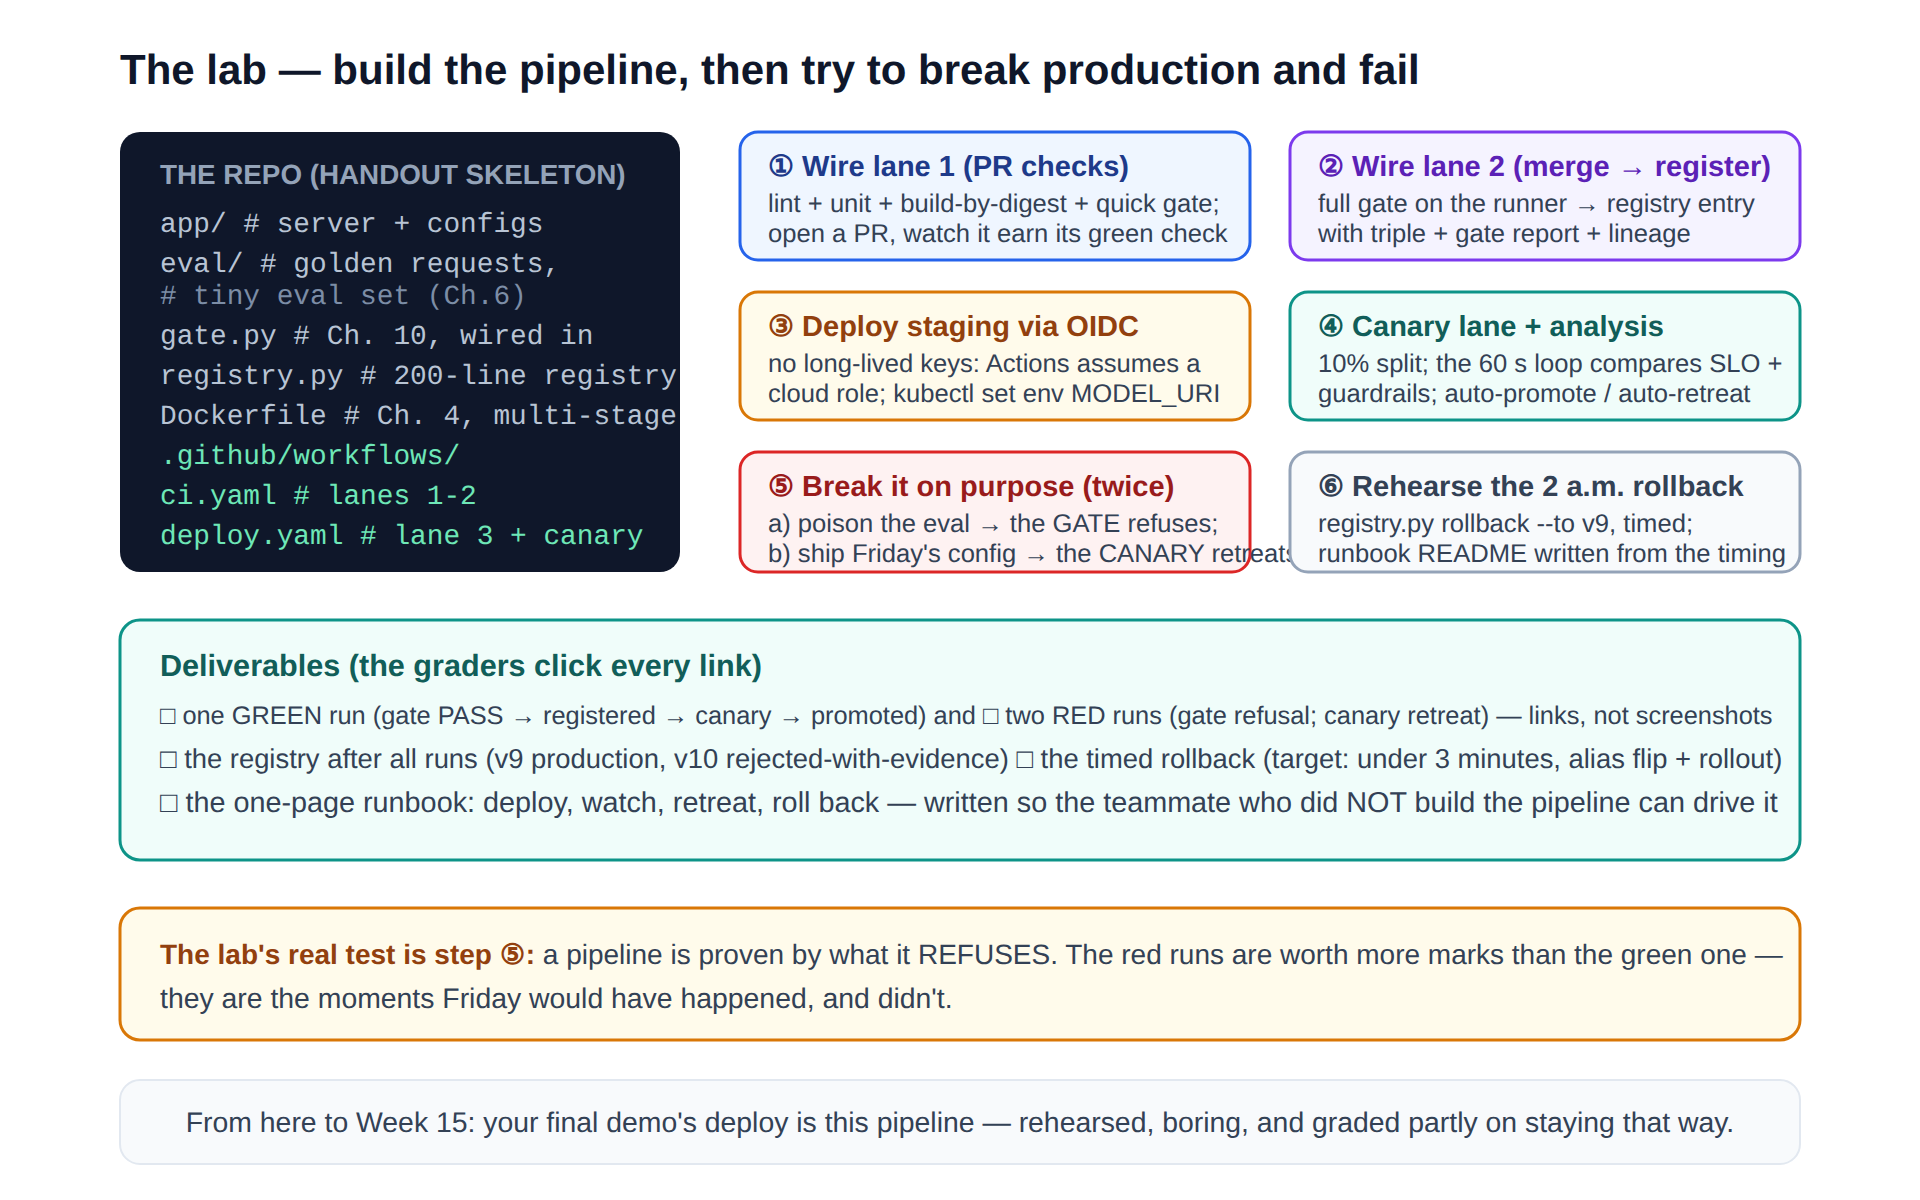
\includegraphics{figures/fig13-7_lab.png}}\\[3pt]
  \figcaption{Figure 13-7  The lab. Left: the repo skeleton — everything this course wrote, now in one tree. Right: six steps from first PR to rehearsed rollback. Bottom: the deliverables are LINKS to runs, and the red runs outrank the green one.}
\end{tbbfigure}

\subsection*{The six steps}

\begin{tbbitemize}
  \item \textbf{① Wire Lane 1.} Fork the skeleton (app/, eval/ with golden requests, gate.py, registry.py, Dockerfile, two workflow files). Open a trivial PR and watch checks run: lint, unit, image build pushed \textbf{by digest}, quick gate (golden requests + 200-sample eval on CPU). Read the logs like Transcript 12-3 — every step should be legible to you now.
  \item \textbf{② Register the runner, wire Lane 2.} The handout script registers your T4 as a self-hosted runner tagged \code{gpu} (one systemd service; spot-friendly). Merge the PR: watch export → equivalence → quantize+calibrate → \textbf{gate} → smoke sweep → \code{registry.py register v10 --stage staging}, and verify the registry entry carries the triple, the gate report, and lineage digests.
  \item \textbf{③ Deploy staging via OIDC.} No long-lived keys anywhere: the workflow assumes a cloud role via OIDC (\code{permissions: id-token: write}), then \code{kubectl set env … MODEL\_URI=\$(registry.py resolve chat/\allowbreak staging)}. Chapter 6's env-var deploy (Transcript 6-7), now typed by a robot with a scoped, minutes-long credential.
  \item \textbf{④ Wire Lane 3 — the canary.} \code{deploy.yaml} patches \code{canaryTrafficPercent: 10} (or the raw-Deployment weighted-Service variant in the handout), then runs the 40-line analysis loop: five 60-second windows, SLO clauses + the guardrail four (answer-length, refusal, format, repetition) vs. the concurrent baseline; verdict → promote (alias flip) or retreat (canary 0\%, PR comment with graphs). Run it green once with a harmless v10.
  \item \textbf{⑤ Break it on purpose, twice.} (a) Poison one golden request's expected format and push: \textbf{the gate refuses in Lane 1} — screenshot the greyed merge button. Revert. (b) Recreate Friday: ship a config with \code{max\_tokens: 256} (the gate passes — it never generates long-form) and promote: \textbf{the canary retreats in window \textasciitilde{}3} on the answer-length guardrail. Save the PR comment — it is Exhibit 13-A, defeated by machinery you built.
  \item \textbf{⑥ Rehearse the 2 a.m. rollback.} With v10 promoted (a good one), run \code{registry.py rollback chat --to v9} and \textbf{time it}: alias flip to first v9-served request. Target under 3 minutes (the floor is §12.3's birth; discuss in the runbook how pre-warm changes it). Write the one-page runbook — deploy, watch, retreat, roll back — such that the teammate who did \textit{not} build the pipeline can drive it. That teammate signs it.
\end{tbbitemize}

\begin{calloutbox}{tbbred}{tbbxFEF2F2}
{\normalsize\bfseries\color{tbbx991B1B}Box 13-1  Deploy red flags — the checklist, published}\par\vspace{3pt}
\begin{tbbitemize}
  \item \textbf{kubectl to production from a laptop} — the pipeline is the only writer; humans write PRs and approvals.
  \item \textbf{A `:latest` (or any re-taggable) reference anywhere on the deploy path} — digests or it didn't happen (Ch. 4, still).
  \item \textbf{A skip-gate flag "for emergencies"} — the emergency path is a faster canary, never a skipped check.
  \item \textbf{Canary without automated analysis} — 10\% traffic that nobody judges is not a canary, it is 10\% of users beta-testing.
  \item \textbf{A rollback that has never been rehearsed} — Friday's twelve minutes were the price of a first rehearsal held in production.
  \item \textbf{Config outside the release} — if changing it doesn't bump a version, it WILL be your Exhibit 13-A.
  \item \textbf{Long-lived cloud keys in repo secrets} — OIDC exists; a leaked key is Knight's eighth server with your logo on it.
\end{tbbitemize}
\end{calloutbox}

\vspace{3.0pt}

\begin{calloutbox}{tbbteal}{tbbxF0FDFA}
{\normalsize\bfseries\color{tbbx115E59}Box 13-2  The runbook, as a template — steal this page}\par\vspace{3pt}
\textbf{DEPLOY} — merge to main; Lane 2 registers vN to staging automatically. To promote: open the promotion PR (\code{registry.py promote chat vN --request}), get one approval, merge — Lane 3 canaries and flips the alias itself. \textit{You never type kubectl.}

\textbf{WATCH} — during canary: the Actions run's live log, or \code{watch registry.py status chat} (shows alias, canary \%, current window verdicts). After promotion: the Ch. 14 dashboard (until then: /metrics + the guardrail script in \code{eval/\allowbreak watch.py}).

\textbf{RETREAT} (canary misbehaving but not yet failed) — \code{gh run cancel <id>} aborts the analysis and zeroes the canary. Safe at any moment; the alias never moved.

\textbf{ROLL BACK} (bad release already promoted) — \code{registry.py rollback chat --to <last-good>} (find it: \code{registry.py list chat} — the previous \code{production} row). Flip ≈ 0.4 s; fleet converges ≈ 2–3 min (§12.3's birth; pre-warm shortens it). Then: file the incident note ON the release's registry entry, and open the fix PR — never patch production by hand.

\textbf{WHO} — promotion approvers: any two of [team list]. 02:00 rule: on-call may roll back alone (rollback is pre-approved by construction — it re-points to a release that already passed everything); promotions wait for daylight.

\textit{Signed by the teammate who did not build the pipeline: \_\_\_\_\_\_\_\_\_\_\_ (the signature is the test).}
\end{calloutbox}

\vspace{3.0pt}

Deliverables: \textbf{links, not screenshots} (graders click) — one green Lane-1→2→3 run ending in a promoted release; the two red runs (gate refusal, canary retreat) with their evidence; the registry listing showing v9 in production, the poisoned candidate rejected-with-evidence; the timed rollback figure; and the signed runbook. Teams that finish early: add a shadow stage for 30 minutes of mirrored traffic and diff the outputs — then read Chapter 14's opening, because the canary's analysis window is about to become permanent and get a name: \textbf{monitoring}.

\begin{calloutbox}{tbbpurple}{tbbpurplefill}
{\normalsize\bfseries\color{tbbpurple}Think About It}\par\vspace{3pt}
\begin{tbbitemize}
  \item Your ⑤(b) canary caught Friday in window 3 (\textasciitilde{}3 minutes). Compute the exposure at 10\% traffic and your measured request rate — then redesign for a paranoid team: what do 1\% first-window, exponential step-up (1→5→25→100) and a 10-window dwell each cost in time-to-full-promotion, and when is the paranoia worth it?
  \item The runbook's rollback floor is the §12.3 birth (\textasciitilde{}150 s). Your teammate proposes keeping the previous release WARM (blue/green style) for one hour post-promotion: price it (§12 arithmetic) and state the rollback time it buys — is the hour the right window? What data from Ch. 14 would tune it?
  \item The lab's registry is 200 lines of JSON in the store. List the first three failure modes at team-scale (concurrent writes? auth? audit tamper?), and which one forces the move to a real registry service first.
  \item Write your project's Lane-3 approval policy: who may approve a promotion, what evidence must the PR show inline (gate report? canary plan? rollback owner?), and what happens at 02:00 when the approver is asleep — encode Knight's lesson without re-creating the two-week release board from §13.1's think-box.
\end{tbbitemize}
\end{calloutbox}

\namedsection{Summary}{The Chapter in Fifteen Points}

\qitem{1}{\textbf{Bad deploys are missing institutions, not careless people.} Exhibit 13-A: a perfect model, a config outside the release, green dashboards, 37 minutes × 100\% of users, and a rollback that required archaeology. Fix the engineer and it repeats; fix versioning + pipeline + exposure and it becomes 0.5 bad user-minutes (74×).}

\qitem{2}{\textbf{Knight Capital is the canonical text:} eight servers deployed by hand, one missed; a reused flag woke dead code; \$460M in 45 minutes — and mid-incident, nobody could say what was running where, so the first fix made it worse. Every §13 heading is one of the SEC order's absences.}

\qitem{3}{\textbf{Frequency is safety, not bravado (Flickr 2009 → DORA):} rare deploys are large, large is unrehearsed, unrehearsed is Knight. The four numbers: lead time (→22 min), deploy frequency (→per merge), blast radius (→10\% with auto-retreat), MTTR (→2-min alias flip). Boring = automated + versioned + gradual + reversible.}

\qitem{4}{\textbf{A release is a TRIPLE with evidence:} weights digest + config digest + image digest, pinned together, gate report stapled on (tolerance, slices, eval-set digest), lineage recorded. Friday's bug — config traveling outside the release — becomes inexpressible.}

\qitem{5}{\textbf{The registry is a database of promises about bytes:} live / safe / changed / who, each answerable in seconds from a cold terminal. Chapter 6 kept the bytes; the registry keeps the meaning. MLflow, the clouds' built-ins — or 200 lines of JSON: the schema is the value.}

\qitem{6}{\textbf{Promotion and rollback are one operation — a pointer move.} Deploys reference aliases (…/prod), never versions; flip 0.4 s, fleet converges via Ch. 5's rollout (\textasciitilde{}2 min, floored by §12.3's birth). Digests, never re-tags (Ch. 4's think-box, answered): tags drift, digests can't.}

\qitem{7}{\textbf{The pipeline is ceremony for checks you already own:} §7.6 equivalence, §10.3's gate, §9.5's sweep, Ch. 6's golden fixtures — run identically on every candidate, with no Friday skip path. In Ch. 5's vocabulary: one more writer of desired state.}

\qitem{8}{\textbf{Model CI ≠ app CI, four ways:} verdicts are tolerances on versioned eval fixtures; artifacts are gigabytes (build once, promote the digest); some stages need silicon (a self-hosted spot-T4 runner); and the last check needs real traffic — which is a strategy, not a test.}

\qitem{9}{\textbf{The red run is the product:} the gate that greys out the merge button is a check with forty green precedents, not a colleague with an opinion — quality disputes become infrastructural. Never skip, never rebuild between check and ship; sign artifacts (cosign/SLSA) from day one.}

\qitem{10}{\textbf{Choose deployment strategies by the question:} rolling — "does it boot?"; blue/green — "can I undo in one second?" (at 2× fleet); canary — "is it broken, judged by reality?"; A/B — "is it better, judged by users?"; shadow — "what would it have done?" (zero risk, 2× compute, stub the side-effects).}

\qitem{11}{\textbf{The canary is Haldane's bird plus the detector that retired it:} 10\% of real traffic, session-hashed (whole conversations); judged against a CONCURRENT baseline; verdict automatic; retreat in seconds. What it checks that the gate cannot: real inputs, real integration (Friday lives here), real infrastructure, real SLOs.}

\qitem{12}{\textbf{Guardrail metrics guard behavior, not goodness:} answer-length, refusal rate, format validity, repetition, language match — cheap proxies for "the model got weird," computable in a 60-second loop. SLO clauses guard the system; guardrails guard the behavior; A/B judges quality.}

\qitem{13}{\textbf{A/B is a product instrument that PRESUMES safety:} days-to-weeks, balanced buckets, pre-registered product metrics, statistics — run only on gated, canaried candidates. Confusing it with a canary buys slow safety and unsound science simultaneously.}

\qitem{14}{\textbf{Managed endpoints are the ladder's last rung:} variants/splits, registries, guardrails as checkboxes — the same concepts at a markup, with less stack control. Price on YOUR utilization (§12.5's ledger); and the gate, fixtures, lineage, SLO sentence, and unit economics never transfer, at any rung.}

\qitem{15}{\textbf{The lab's grading is the chapter's thesis:} one green run, two red runs (gate refusal, canary retreat), a timed rehearsed rollback, and a runbook a non-author can drive. A pipeline is proven by what it refuses — the red runs are Fridays that didn't happen.}

\namedsection{Exercises}{}

\subsection*{A. Multiple choice}

\qitem{1}{Exhibit 13-A's bug (max\_tokens=256) survived the offline gate because:}

\begin{tbboptions}
  \item ① The gate's tolerance was too loose        ② The gate scores teacher-forced eval and never generates with the SHIPPED config — it tested the model, not the release
  \item ③ The eval set was too small        ④ The gate ran on the wrong GPU
\end{tbboptions}

\qitem{2}{A "release" in this chapter's sense is:}

\begin{tbboptions}
  \item ① The model weights        ② The Docker image
  \item ③ The pinned triple — weights + config + image digests — with its gate report and lineage        ④ Whatever the prod alias points at
\end{tbboptions}

\qitem{3}{Rollback via registry alias is fast and safe primarily because:}

\begin{tbboptions}
  \item ① It skips the readiness probes        ② The decision, the knowledge (what is safe), and the mechanism are one rehearsed pointer move — convergence is the ordinary Ch. 5 rollout
  \item ③ It avoids pulling images        ④ Aliases bypass the LB
\end{tbboptions}

\qitem{4}{Knight Capital's first remediation (rolling back the new code on the seven good servers) made things worse because:}

\begin{tbboptions}
  \item ① The rollback was too slow        ② The trigger was the reused FLAG plus dead code on the un-updated eighth server — nobody had an authoritative picture of what ran where
  \item ③ The market moved against them        ④ The new code was actually fine
\end{tbboptions}

\qitem{5}{Model CI builds artifacts once and promotes digests across environments because:}

\begin{tbboptions}
  \item ① Rebuilding is slow        ② Any rebuild between check and ship un-checks everything — the gated bytes must BE the shipped bytes
  \item ③ Registries charge per build        ④ Digests compress better
\end{tbboptions}

\qitem{6}{The canary judges against a concurrent baseline rather than yesterday's metrics because:}

\begin{tbboptions}
  \item ① Yesterday's data is deleted        ② Traffic has a diurnal personality (Ch. 12) — only a same-time control isolates the release from the hour
  \item ③ Prometheus retention is short        ④ Baselines drift due to autoscaling
\end{tbboptions}

\qitem{7}{Canary vs. A/B, correctly stated:}

\begin{tbboptions}
  \item ① They are synonyms        ② Canary is safety (minutes, "is it broken?", automatic verdict); A/B is product (weeks, "is it better?", statistics) — and A/B presumes gate + canary already passed
  \item ③ A/B is for infrastructure, canary for models        ④ Canary needs more traffic than A/B
\end{tbboptions}

\qitem{8}{Shadow deployment's two non-negotiable costs are:}

\begin{tbboptions}
  \item ① Slower rollouts and bigger images        ② User-visible risk and pager load
  \item ③ \textasciitilde{}2× compute for the mirrored slice, and stubbing every side-effect (writes, billing, emails)        ④ Extra registries and longer gates
\end{tbboptions}

\subsection*{B. Short answer}

\qitem{1}{Name the three missing institutions of Exhibit 13-A and the section that builds each.}

\qitem{2}{Why must the eval set itself be a versioned, digest-pinned fixture? What silently breaks if someone "just adds a few hard examples" to it in place?}

\qitem{3}{List the three lanes of the model pipeline with their triggers, runners, and end states.}

\qitem{4}{Give four guardrail metrics for a generative canary and the one-sentence rationale for guardrails as a class ("sameness of behavior").}

\qitem{5}{Why are canary splits session-hashed for chat workloads — name both the UX failure and the metrics failure of per-request splits.}

\qitem{6}{State the emergency-deploy rule ("never skip the gate — the emergency path is a faster canary") and what Knight's incident contributes to its justification.}

\subsection*{C. Essay}

\qitem{1}{The postmortem essay: write Exhibit 13-A's blameless postmortem — timeline, impact (bad user-minutes), root causes stated as missing institutions (never as names), and remediation mapped to §§13.2–13.4 with owners and dates. Then add the paragraph most postmortems omit: which remediation you would NOT do, and why (cost vs. recurrence).}

\qitem{2}{Defend or attack: "The registry is the load-bearing institution; the pipeline and canary are automation around it." Use Friday (could a registry alone have saved it?), Knight (what did they lack FIRST?), and the 2 a.m. test — then state which single institution you would build first at a startup, and the failure you accept by deferring the others.}

\qitem{3}{The strategy-design essay: your team ships (a) weekly base-model upgrades, (b) daily prompt/config tweaks, (c) a quarterly engine major-version. For each: the full path (lanes, strategy rungs, dwell times, guardrails), the blast-radius arithmetic, and the rollback plan with its floor. Justify every place your three paths differ.}

\qitem{4}{The build-vs-buy essay, deployment edition: compare your Lane 1–3 pipeline targeting KServe against SageMaker endpoints with registry + guardrails, for YOUR project team (size, models, traffic from the midpoint review). Price the markup with §12.5's ledger, list what transfers unchanged (the triple, gate, fixtures), and end with the memo: adopt, defer, or hybrid — and the single metric that would flip your answer.}

\namedsection{Answers and Commentary}{}

\subsection*{A. Multiple choice}

\qitem{1}{\textbf{②} The gate's blind spot was structural: it evaluated weights, but the failure lived in the release (weights + CONFIG as deployed). "Test what you ship" — which is why Lane 2 gates the assembled release and §13.4 still canaries it. (§13.1, §13.3)}

\qitem{2}{\textbf{③} ④ is circular (the alias points at a release; it doesn't define one) — the triple + evidence is the unit that travels, and its pinning is what made Friday's class of bug inexpressible. (§13.2)}

\qitem{3}{\textbf{②} Speed matters less than the rehearsed unity: decision + knowledge + mechanism in one place. The fleet-side floor is §12.3's birth, which is why the runbook times it. (§13.2)}

\qitem{4}{\textbf{②} The lesson is epistemic, not procedural: without an authoritative "what runs where," remediation is guesswork — and their guess re-armed the trigger. The registry is that authority. (§13.1–13.2)}

\qitem{5}{\textbf{②} Identity through the pipeline is the whole trust chain: gate → registry → deploy must reference the same digests, or the green check certifies bytes that never ship. (§13.3)}

\qitem{6}{\textbf{②} Ch. 12's diurnal curve is a confounder: 14:00-vs-03:00 comparisons measure the clock, not the candidate. Concurrent control is the cheapest valid experiment design. (§13.4)}

\qitem{7}{\textbf{②} Different instruments for different questions; the ordering (gate → canary → A/B) is safety before science. (§13.4)}

\qitem{8}{\textbf{③} The mirrored slice consumes real inference (Ch. 12 prices it) and a shadow with live side-effects is a second production, not a rehearsal. (§13.4)}

\subsection*{B. Short answer}

\qitem{1}{Versioned releases (§13.2 — the registry and the triple); a pipeline that tests what ships (§13.3 — the three lanes); gradual exposure with automatic retreat (§13.4 — the canary). (§13.1)}

\qitem{2}{The gate's verdict is "Δ vs. tolerance ON this set" — the set is half the measurement. Mutating it in place silently changes the meaning of every historical PASS/FAIL (grades on a different exam), breaks regression comparisons, and un-pins lineage. New examples → new eval-set version, re-baseline explicitly. (§13.3)}

\qitem{3}{Lane 1: every PR / CPU runners / hygiene + quick gate → green check. Lane 2: merge to main / self-hosted GPU runner / export→quantize→GATE→smoke → a registered staging release with evidence. Lane 3: human approval / cluster via OIDC / canary analysis → auto-promote (alias flip) or auto-retreat. (§13.3)}

\qitem{4}{Answer-length distribution, refusal/apology rate, format validity (JSON parses), repetition score (+ language match). Rationale: a deploy's null hypothesis is behavioral SAMENESS — guardrails detect "got weird" cheaply while true quality judgment waits for A/B. (§13.4)}

\qitem{5}{UX: a conversation split across models flickers personality mid-thread. Metrics: per-request mixing contaminates both populations (the same session's turns land in both arms), destroying the comparison's independence. Hash the conversation id (Ch. 11's affinity machinery). (§13.4)}

\qitem{6}{Emergencies change SPEED (shorter canary windows, pre-staged rollback, wider paging), never CHECKS — because pressure is precisely when unverified change is deadliest: Knight's deploy was a deadline rush, manual, unverified, and un-rolled-back-able. (§13.3, §13.1)}

\subsection*{C. Essay (grading points)}

\qitem{1}{Look for: minute-level timeline with the two innocent-looking green checkpoints (probes, dashboards); impact in bad user-minutes (37) not vibes; causes as institutions with the config-outside-release named precisely; remediations mapped to sections with the canary's guardrail called out as the class-catcher; and a defensible "won't do" (e.g., full blue/green — priced against §12 and rejected for a canary at near-zero marginal cost). Blamelessness that still assigns OWNERSHIP of fixes earns the top band. (§§13.1–13.4)}

\qitem{2}{Strong essays notice the instruments answer different failure classes: the registry is the epistemic floor (Knight's missing "what runs where"), but Friday needed the canary (the registry records a bad release beautifully). First-build defenses: registry (cheapest, enables rehearsed rollback) vs. canary (largest bad-user-minute reduction per effort) both earn credit if the deferred failure is stated honestly — e.g., registry-first accepts one more Friday; canary-first accepts slow rollbacks. (chapter-wide)}

\qitem{3}{Expect three genuinely different paths: (a) shadow at the family boundary + long canary + full A/B for quality claims; (b) Lane 1 + rolling or fast canary (config class — but Exhibit 13-A demands the guardrail canary stays!); (c) blue/green for the engine (instant undo, infra-shaped risk, priced 2× window via §12) + shadow for numerics (§7.6/§10.4 re-order caveat). Reward explicit dwell times, blast-radius numbers, and rollback floors (§12.3) rather than strategy name-dropping. (§13.4)}

\qitem{4}{The ledger must appear (markup × instance-hours vs. SRE-time saved), the transferable artifacts named (triple, gate, fixtures, registry schema — and the pipeline's Lanes 1–2 unchanged; only Lane 3's verbs swap to vendor APIs), and the verdict tied to team shape. The flipping metric done well: models×teams growth (→managed earlier), utilization at scale (→self-host), or a compliance requirement. Any decision earns full credit with consistent arithmetic; brochure-quoting earns none. (§13.5, §12.5)}

\namedsection{Further Reading}{}

Entries tagged \textbf{[This week]} support the lab directly; \textbf{[Wk N]} marks material that pays off later.

\begin{tbbitemize}
  \item \textbf{[This week] GitHub Actions docs — workflow syntax, self-hosted runners, OIDC to cloud providers} — the lab's three load-bearing pages; the OIDC guide retires the last long-lived key in your project.
  \item \textbf{[This week] MLflow Model Registry documentation (aliases, stages, lineage)} — Chapter 6's further reading, now due: the registry schema behind Transcript 13-1, with a UI. Read it as schema, not as product.
  \item \textbf{[This week] Argo Rollouts documentation (canary, analysis templates)} — Chapter 5's promised continuation: step-weights, Prometheus-backed analysis, auto-rollback — §13.4 as a controller.
  \item \textbf{SEC Administrative Order re: Knight Capital (2013) — and the "Knightmare" postmortem literature} — the primary text of §13.1; read the order's findings against Figure 13-3 and count the absent lanes.
  \item \textbf{J. Allspaw \& P. Hammond, "10+ Deploys per Day: Dev and Ops Cooperation at Flickr" (Velocity 2009)} — the talk that seeded DevOps; watch it (it survives online) noticing how many 2009 pains this course's chapters have since institutionalized.
  \item \textbf{Google SRE Workbook — "Canarying Releases"} — the mature treatment of §13.4: population selection, metric choice, and the statistics of small canaries; the guardrail-vs-SLO distinction, at production depth.
  \item \textbf{DORA — "Accelerate: State of DevOps" reports} — the measurement program behind §13.1's four numbers; useful as a mirror: score the course project honestly and find your weakest key.
  \item \textbf{[This week, fun] The Actions tab of any large OSS model repo (vLLM itself is instructive)} — read one green and one red run end to end; you now speak the language. Notice what they gate, and what they still deploy by hand.
\end{tbbitemize}

\vspace{5.0pt}

\begin{calloutbox}{tbbblue}{tbbbluefill}
{\normalsize\bfseries\color{tbbblue}Next chapter — Chapter 14: Monitoring and Reliability}\par\vspace{3pt}
The canary's analysis loop ran for five windows and shut off — but the questions it asked ("is TTFT honest? did behavior drift?") do not expire at promotion; production keeps answering them forever, to an audience of nobody. Chapter 14 makes the audience permanent: \textbf{Prometheus and Grafana} turn Chapter 11's /metrics lines and this chapter's guardrails into the serving dashboard the syllabus promises, \textbf{alerting} encodes the SLO sentence so pages fire on burn rates rather than vibes, and \textbf{drift detection} watches the one thing no deploy gate can freeze — the input distribution itself, wandering away from your eval sets one user cohort at a time. Plus the war story §12.4 scheduled: the time-sliced GPU's unexplainable p99, solved on a dashboard, live. The lab builds the dashboard and its alarms — and the on-call shift that inherits your pipeline finally gets its instrument panel.
\end{calloutbox}
